\documentclass[11pt,a4paper]{article}

% --- PACKAGES ---
\usepackage[utf8]{inputenc}
\usepackage[T1]{fontenc}
\usepackage[english]{babel}
\usepackage{geometry}
\geometry{margin=1in}
\usepackage{setspace}
\onehalfspacing
\usepackage{amsmath,amssymb,amsthm,mathtools}
\usepackage{graphicx}
\usepackage{xcolor}
\usepackage{hyperref}
\usepackage{natbib}
\usepackage{mdframed}
\usepackage{booktabs}
\usepackage{filecontents}
\usepackage{enumitem}
\usepackage{float}
\usepackage{caption}
\usepackage{subcaption}

% --- CUSTOM COMMANDS ---
\newcommand{\SYSTEM}{\textbf{SYSTEM}}
\newcommand{\SES}{\textbf{SES}}
\newcommand{\betaDehum}{$\beta$-dehumanization}
\newcommand{\CC}{$\mathcal{C}$}
\newcommand{\CU}{$\mathcal{C}_U$}
\newcommand{\Fall}{\textit{Fall}}
\newcommand{\Love}{$\mathcal{L}$}
\newcommand{\Suffering}{$\mathcal{S}$}

% --- COLORS ---
\definecolor{sveblue}{RGB}{0, 51, 102}
\definecolor{sveteal}{RGB}{0, 102, 153}
\definecolor{svered}{RGB}{204, 0, 0}
\definecolor{sokratesblue}{RGB}{41, 128, 185}
\definecolor{solomongold}{RGB}{243, 156, 18}
\definecolor{ivangreen}{RGB}{39, 174, 96}

% --- HYPERREF SETUP ---
\hypersetup{
    colorlinks=true,
    linkcolor=sveblue,
    citecolor=sveteal,
    urlcolor=sokratesblue,
    pdftitle={S.V.E. XII: SYSTEM — Geometry of the Fall and the Path to Collective Awareness},
    pdfauthor={Dr. Artiom Kovnatsky et al.}
}

% --- THEOREM ENVIRONMENTS ---
\theoremstyle{definition}
\newtheorem{definition}{Definition}[section]
\newtheorem{axiom}{Axiom}[section]
\newtheorem{proposition}{Proposition}[section]
\newtheorem{parameter}{Parameter}[section]
\theoremstyle{remark}
\newtheorem{remark}{Remark}[section]
\newtheorem{example}{Example}[section]

% --- BIBLIOGRAPHY ---
\begin{filecontents*}{\jobname.bib}
@book{smith1776wealth,
  title={An Inquiry into the Nature and Causes of the Wealth of Nations},
  author={Smith, Adam},
  year={1776},
  publisher={W. Strahan and T. Cadell}
}

@article{dzendialogue,
    title={Dzen-studio | Training-Article: Seeds or Capitalism 2.0},
    author={Kovnatsky, Artiom},
    year={2025}
}

@misc{spe,
    author = {Haney, C. and Banks, W. C. and Zimbardo, P. G.},
    year = {1973},
    title = {A study of prisoners and guards in a simulated prison},
    howpublished = {Naval Research Reviews}
}

@book{jung_collective_unconscious,
    author = {Jung, Carl G.},
    title = {The Archetypes and the Collective Unconscious},
    series = {Collected Works Vol. 9 Part 1},
    year = {1969},
    publisher = {Princeton University Press}
}

@book{plato_republic,
    author = {Plato},
    title = {The Republic},
    year = {-380},
    note = {Allegory of the Cave}
}

@misc{einstquote,
    author={Einstein, Albert},
    note={Quote on rational knowledge and spiritual evolution}
}

@book{pereslegin_summa,
    author = {Pereslegin, Sergey B.},
    title = {Summa Strategiae},
    year = {2005},
    publisher = {AST}
}

@book{machiavelli_prince,
    author = {Machiavelli, Niccolò},
    title = {The Prince},
    year = {1532}
}

@book{sun_tzu_art_of_war,
    author = {Sun Tzu},
    title = {The Art of War}
}

@misc{russell_quote,
    author = {Russell, Bertrand},
    title = {On Education and Critical Thinking},
    year = {1950}
}

@article{sve0,
    author = {Kovnatsky, Artiom},
    title = {S.V.E. 0: Self-Information-Purification and Epistemological Boxing},
    year = {2020-2024}
}

@article{sve4,
    author = {Kovnatsky, Artiom},
    title = {S.V.E. IV: Christ-Vector and Geodesic Ethics},
    year = {2021}
}

@article{sve8,
    author = {Kovnatsky, Artiom},
    title = {S.V.E. VIII: Mathematical Formalization of Love and Suffering},
    year = {2022}
}

@article{sve9,
    author = {Kovnatsky, Artiom},
    title = {S.V.E. IX: Verification and Falsification Framework},
    year = {2023}
}

@article{sve10,
    author = {Kovnatsky, Artiom},
    title = {S.V.E. X: Cognitive Operating System},
    year = {2023}
}

@article{sve11,
    author = {Kovnatsky, Artiom},
    title = {S.V.E. XI: Verifiable Knowledge Base},
    year = {2024}
}
\end{filecontents*}

% --- DOCUMENT START ---
\begin{document}

% --- TITLE PAGE ---
\begin{titlepage}
\centering
\vspace*{1cm}

{\Huge\bfseries S.V.E. XII: \SYSTEM{}}\\[0.5cm]
{\Large Diagnosis of Collective Unconscious Dynamics}\\[0.3cm]
{\Large The Geometry of the Fall and the Response-Path}\\[0.3cm]
{\Large to Collective Awareness}\\[2cm]

{\large\textit{Integrating Jung's Unconscious, Smith's Invisible Hand,}\\[0.2cm]
\textit{and Plato's Cave within the S.V.E. Framework}}\\[3cm]

{\large Dr. Artiom Kovnatsky}\\[0.5cm]
{\normalsize with contributions from the S.V.E. community}\\[2cm]

{\large\today}\\[0.5cm]
{\normalsize Version 0.7 — Open for Verification and Critique}\\[1cm]

\vfill

\begin{mdframed}[backgroundcolor=gray!5]
\small
\textbf{Abstract:} This paper presents \SYSTEM{} (Socio-Economic System Transforming Minds) as a comprehensive model of collective unconscious dynamics that emerge from and perpetuate socio-economic structures. Building on Jung's collective unconscious, Smith's invisible hand, and Plato's Cave allegory, we provide a geometric formalization of how humanity's metaphorical "Fall" from unity continues to shape modern society through invisible, systemic forces. We formalize the \SES{} (Socio-Economic System) parameters, demonstrate their historical evolution, and reveal how digitization accelerates inequality dynamics. The paper introduces formal axioms, propositions, and a path toward collective awareness through S.V.E. protocols, including the PEMY business model as a practical implementation of "Capitalism 2.0." This work synthesizes insights from previous S.V.E. papers (0-XI) into an integrated diagnostic and therapeutic framework for understanding and transforming systemic dehumanization.
\end{mdframed}

\end{titlepage}

% --- TABLE OF CONTENTS ---
\tableofcontents
\newpage

% --- EPIGRAPHS ---
\section*{Opening Reflections}
\addcontentsline{toc}{section}{Opening Reflections}

\begin{mdframed}[backgroundcolor=gray!10]
\textit{"Some children have a habit of thinking—one of the purposes of education is to rid them of it. Uncomfortable questions are silenced, even punished. Collective emotions are used to instill the needed views, especially of a nationalist kind. Capitalists, militarists, and churchmen collaborate in education because it is advantageous to all of them that people develop an emotional attitude toward reality rather than critical thinking."}

--- \textbf{Bertrand Russell}, British philosopher, logician, mathematician, and Nobel Prize laureate in Literature (1950)
\end{mdframed}

\vspace{0.5cm}

\begin{mdframed}[backgroundcolor=gray!10]

\textit{"The further the spiritual evolution of mankind advances, the more certain it seems to me that the path to genuine religiosity does not lie through the fear of life, and the fear of death, and blind faith, but through striving after rational knowledge."}

--- \textbf{Albert Einstein} \cite{einstquote}
\end{mdframed}

\newpage

% ==========================================
% PART I: THE SYSTEM HYPOTHESIS
% ==========================================

\section{Part I: The \SYSTEM{} Hypothesis — A Geometric Model of Collective Dynamics}

\subsection{Introduction: The Invisible Architecture}

We live within systems that shape our thoughts, desires, and behaviors in ways that remain largely invisible to us. From the moment we are born, we are embedded in socio-economic structures (\SES{}) that determine not only our material conditions but also the very fabric of our consciousness. Like prisoners in Plato's Cave \cite{plato_republic}, we mistake the shadows on the wall for reality itself, unaware of the mechanisms casting those shadows.

This paper proposes \SYSTEM{} (\textbf{S}ocio-\textbf{E}conomic \textbf{S}ystem \textbf{T}ransforming \textbf{M}inds) as a formal model for understanding these invisible dynamics. \SYSTEM{} is not a conspiracy—it is an emergent property of human systems, rooted in what Carl Jung called the "collective unconscious" \cite{jung_collective_unconscious} and manifesting through what Adam Smith termed the "invisible hand" \cite{smith1776wealth}.

\begin{figure}[H]
    \centering
    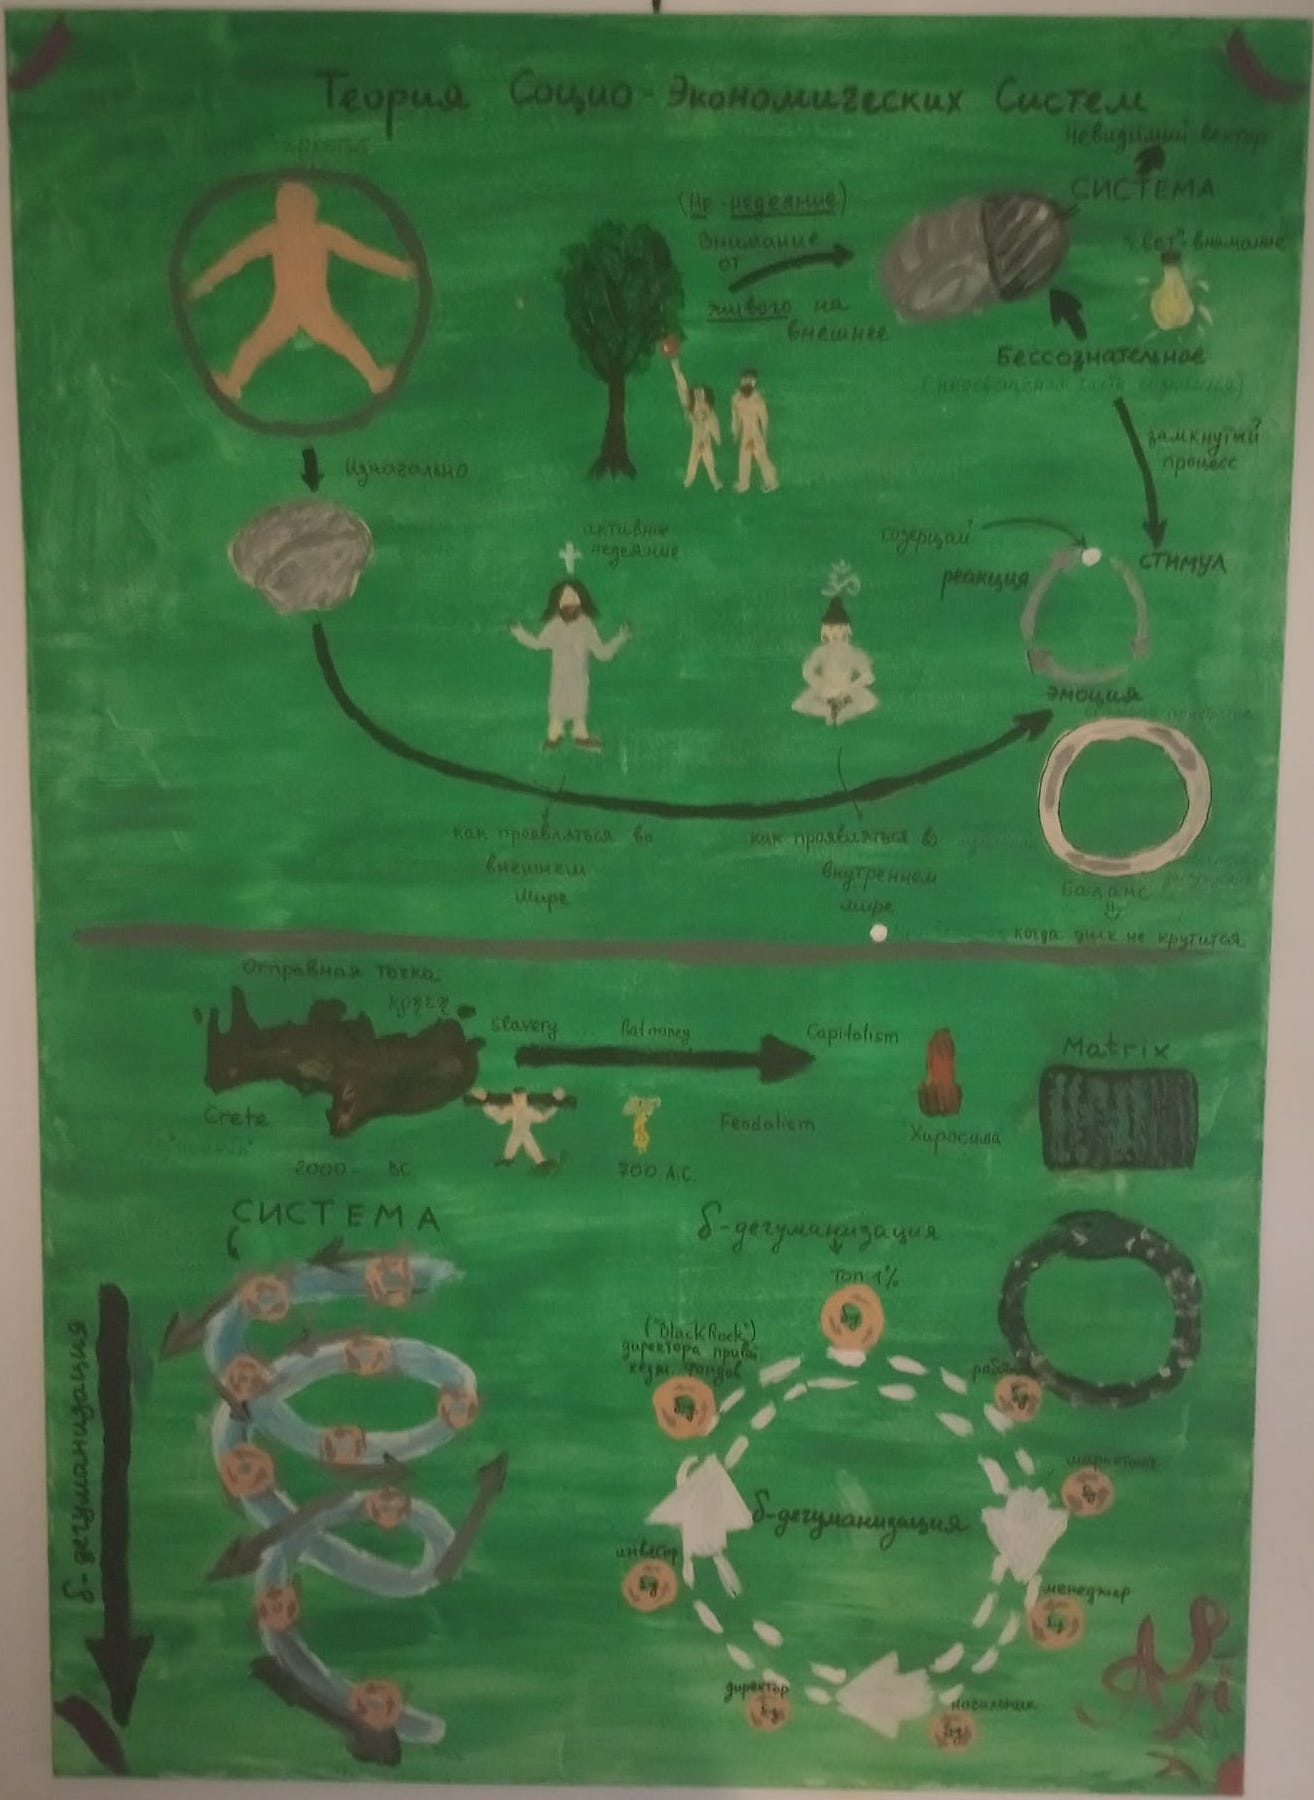
\includegraphics[width=0.85\textwidth]{fig/theory.jpeg}
    \caption{\textbf{The S.V.E. Theoretical Framework}: This illustration synthesizes the core elements of the S.V.E. universe. At the foundation lies the geometric manifold \CC{} (Consciousness Space), depicted as a curved surface representing the terrain of human consciousness. The "Fall" is geometrically modeled as a distortion in this manifold—a region of high curvature where geodesics (paths of love and truth) are bent away from their optimal trajectories. 
    
    The diagram shows three key layers: (1) \textbf{The Individual Level} — where the Cognitive Operating System (S.V.E. X) operates, showing the interplay between conscious awareness (light) and unconscious patterns (shadow); (2) \textbf{The Collective Level} — where \SES{} parameters (П1-П5) shape the manifold's geometry through economic incentive structures, creating attractor basins that pull individuals toward dehumanizing behaviors; (3) \textbf{The Meta Level} — where \SYSTEM{} emerges as an autonomous dynamic, feeding on \betaDehum{} cycles.
    
    Key mechanisms illustrated include: the dopamine feedback loops creating the Fall's gravitational pull; the "Invisible Hand" operating through collective unconscious patterns; Plato's Cave allegory mapped onto consciousness manifold regions (lit vs. shadowed); and the Christ-Vector geodesics pointing toward paths of healing and integration. The Verifiable Knowledge Base (VKB) is shown as a lighthouse illuminating previously dark regions of the manifold, while PEMY business models represent structural interventions that reshape the manifold's curvature itself. This is the map for navigating from fragmentation toward wholeness.}
    \label{fig:theory}
\end{figure}

\subsection{Historical Context and Synthesis}

The concept of invisible forces shaping society is not new:

\begin{itemize}[leftmargin=*]
\item \textbf{Adam Smith (1776)} described how individual self-interest, mediated by market mechanisms, produces collective outcomes—the "invisible hand" \cite{smith1776wealth}. However, Smith assumed rational actors and benign outcomes, failing to anticipate how concentrated capital and information asymmetry could distort this mechanism.

\item \textbf{Carl Jung (1940s)} proposed the "collective unconscious"—shared psychological patterns inherited across humanity, manifesting as archetypes, shadows, and unconscious drives \cite{jung_collective_unconscious}. Jung recognized that much of human behavior is driven by forces below the threshold of awareness.

\item \textbf{Plato (380 BCE)} offered the Cave allegory \cite{plato_republic}: prisoners mistake shadows for reality because they cannot turn to see the fire casting those shadows. The allegory speaks to humanity's tendency to confuse constructed representations with truth itself.
\end{itemize}

\textbf{The S.V.E. Synthesis:} \SYSTEM{} integrates these insights into a unified geometric model. We propose that:

\begin{enumerate}
\item The collective unconscious (\CU{}) is not merely psychological but is \textit{instantiated} and \textit{reinforced} by socio-economic structures.
\item The "invisible hand" operates not in a vacuum of pure economics, but through psychological dynamics embedded in \SES{}.
\item The "shadows on the wall" are cast by \SYSTEM{} dynamics, and escaping the Cave requires not just individual enlightenment but \textit{systemic transformation}.
\end{enumerate}

\subsection{Core Definitions and Formalism}

We now introduce the formal structure of \SYSTEM{}.

\begin{definition}[Consciousness Manifold \CC{}]
\label{def:consciousness_manifold}
The \textbf{Consciousness Manifold} \CC{} is a geometric space representing the possible states of human consciousness—individual and collective. Points on \CC{} correspond to cognitive-emotional-behavioral configurations. The manifold has:
\begin{itemize}
\item \textbf{Metric structure} $g_{\mu\nu}$: defines "distance" between states (how easy/hard it is to transition)
\item \textbf{Curvature} $R_{\mu\nu\rho\sigma}$: represents systemic distortions that bend trajectories
\item \textbf{Lit regions}: areas of conscious awareness ("vnimanie eto svet — attention is light" — attention is light)
\item \textbf{Shadow regions}: unconscious areas (Jungian shadow, Platonic shadows)
\end{itemize}
\end{definition}

\begin{figure}[H]
    \centering
    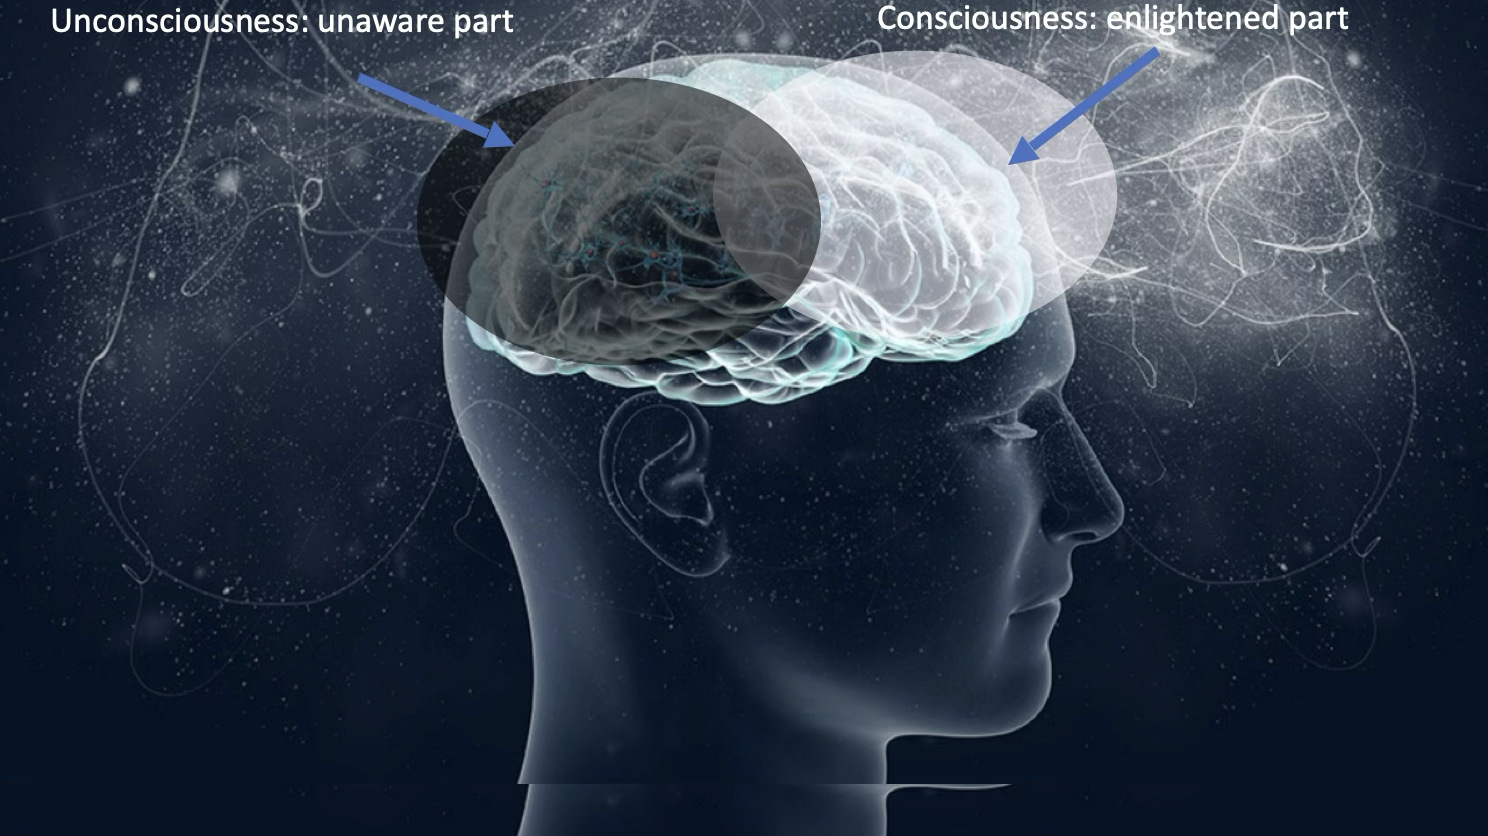
\includegraphics[width=0.65\textwidth]{fig/conciousness_subconciousness_model_eng.png}
    \caption{\textbf{Model of Consciousness and the Unconscious}: The human mind as a manifold where attention (light) illuminates certain regions while vast territories remain in darkness (unconscious). The Fall creates a persistent shadow region that resists illumination. \SYSTEM{} operates primarily in these shadow regions, shaping behavior below the threshold of awareness.}
    \label{fig:conscious_unconscious}
\end{figure}

\begin{definition}[\betaDehum{} — Beta-Dehumanization]
\label{def:beta_dehum}
\betaDehum{} is the process by which individuals or groups are subtly reduced in perceived moral worth, humanity, or agency through \textit{systemic mechanisms} rather than overt violence. It manifests as:
\begin{itemize}
\item Cognitive distancing ("us vs. them")
\item Moral disengagement (rationalizing harm as necessary/inevitable)
\item Transactional reduction (viewing people as resources, metrics, or obstacles)
\item Empathy suppression (deadening emotional response to suffering)
\end{itemize}
Unlike overt dehumanization, \betaDehum{} is often invisible to both perpetrator and victim, embedded in "normal" institutional practices.
\end{definition}

\begin{definition}[The Fall — Operational Definition]
\label{def:fall}
In the S.V.E. framework, the \textbf{Fall} is not a supernatural event but an \textit{operationally defined} transition in human consciousness characterized by:

\begin{enumerate}
\item \textbf{Fragmentation}: Split between conscious self and unconscious shadow (Jung)
\item \textbf{Dopamine Hijacking}: Pursuit of pleasure/avoidance of pain becomes dominant driver, overriding love-based values
\item \textbf{Trauma Imprint}: Collective memory of suffering creating fear-based reactive patterns
\item \textbf{Illusion Fixation}: Attachment to shadows (Plato) rather than underlying reality
\end{enumerate}

Geometrically, the Fall introduces \textit{curvature distortions} in \CC{}, bending geodesics (optimal paths) away from love (\Love{}) and truth toward ego-protection and \betaDehum{}.
\end{definition}

\begin{remark}
The term "Fall" is used metaphorically, drawing on religious and mythological narratives familiar across cultures (Genesis, Prometheus, etc.), but we \textit{strip away} supernatural claims and \textit{operationalize} it as a phase transition in human cognitive-behavioral patterns. This transition is \textit{reversible} through awareness and systemic change.
\end{remark}

\subsection{The Three Foundational Axioms of \SYSTEM{}}

\begin{axiom}[Unconscious Primacy]
\label{ax:unconscious_primacy}
The majority of human behavior and decision-making is driven by \textit{unconscious} processes—patterns, fears, desires, and cognitive biases that operate below the threshold of awareness. Conscious thought is often a post-hoc rationalization of unconscious drives.

\textbf{Evidence base:} Modern neuroscience (e.g., Kahneman's System 1/System 2 \cite{kahneman}), psychoanalysis (Freud, Jung), behavioral economics (predictable irrationality \cite{ariely}), and the Stanford Prison Experiment \cite{spe} demonstrating situational power over conscious values.
\end{axiom}

\begin{axiom}[Socio-Economic Embedding]
\label{ax:ses_embedding}
Unconscious patterns (\CU{}) are not purely innate but are \textit{shaped, reinforced, and transmitted} through socio-economic structures (\SES{}). The parameters of \SES{}—incentive structures, resource distribution, power hierarchies—act as the "training environment" for collective consciousness.

\textbf{Implication:} To change consciousness, we must change \SES{} parameters. Individual awakening is necessary but insufficient; systemic reform is required.
\end{axiom}

\begin{axiom}[Emergent Autonomy of \SYSTEM{}]
\label{ax:emergent_autonomy}
Once established, \SYSTEM{} exhibits \textit{quasi-autonomous} dynamics. It perpetuates itself through:
\begin{itemize}
\item Self-reinforcing feedback loops (the rich get richer, power concentrates)
\item Capture of institutions (education, media, politics)
\item Resistance to disruption (immune response to threats)
\end{itemize}

\textbf{Analogy:} Like an artificial intelligence that optimizes for a misaligned objective function, \SYSTEM{} "optimizes" for its own perpetuation, even when this conflicts with human flourishing.
\end{axiom}

\begin{remark}[On Conspiracy vs. Emergence]
\SYSTEM{} is \textit{not} a conspiracy in the traditional sense—there is no secret cabal pulling all strings. Rather, it is an \textit{emergent property} of millions of unconscious actors operating within structures that reward certain behaviors and punish others. However, within \SYSTEM{}, there \textit{are} actors who consciously exploit its dynamics for advantage (e.g., leveraging information asymmetry, regulatory capture). The key insight is that \textit{most participants, including elites, are unconscious of the full picture}—they are "hostages" of the system they perpetuate.
\end{remark}

\subsection{The \SES{} Parameters: Formalizing Socio-Economic Structures}

To make \SYSTEM{} dynamics concrete, we introduce five key parameters that characterize any \SES{}:

\begin{parameter}[П1: Incentive Alignment]
\label{param:incentive}
\textbf{Definition:} The degree to which the reward structure of the system aligns individual behavior with collective well-being.

\textbf{Spectrum:}
\begin{itemize}
\item \textbf{Highly Misaligned} (current capitalism): Rewards extraction, exploitation, short-term profit maximization at the expense of long-term sustainability and human welfare.
\item \textbf{Aligned} (proposed PEMY model): Rewards cooperation, transparency, and holistic value creation (including well-being, ecological health, not just profit).
\end{itemize}

\textbf{Mathematical Model:}
Let $U_i$ be individual utility and $W$ be collective welfare. Define alignment as:
\[
A = \frac{\text{Cov}(U_i, W)}{\sqrt{\text{Var}(U_i) \cdot \text{Var}(W)}}
\]
where $A \in [-1, 1]$. Current systems often have $A < 0$ (anti-correlated), while ideal systems approach $A \to 1$.
\end{parameter}

\begin{parameter}[П2: Resource Distribution]
\label{param:resource}
\textbf{Definition:} The concentration vs. dispersion of wealth, power, and access to resources.

\textbf{Measurement:} Gini coefficient, wealth percentile ratios (e.g., top 1\% vs. bottom 99\%).

\textbf{Dynamics:} Under current \SES{}, П2 shows accelerating concentration:
\begin{itemize}
\item 1980: Top 1\% held $\sim$10\% of wealth (US)
\item 2024: Top 1\% holds $\sim$35\% of wealth (US)
\item COVID-19: Top billionaires gained \$637B in 3 months while 40M lost jobs
\end{itemize}

\textbf{Thought Experiment:}
\begin{example}
Imagine 100 people and 100 coins. Initially: 54 coins belong to 1 person, 31 coins to the next 19 people, 15 coins to the remaining 80.

Assume:
\begin{itemize}
\item Top 1\% earns 10\% ROI annually
\item Money supply grows 3\% annually
\item Bottom 99\% split the growth minus top 1\% gains
\end{itemize}

Evolution:
\begin{align*}
\text{Year 0:} & \quad \text{Top 1\% = 54, Bottom 99\% = 46} \\
\text{Year 1:} & \quad \text{Top 1\% = 59.4, Bottom 99\% = 45.6} \\
\text{Year 2:} & \quad \text{Top 1\% = 65.34, Bottom 99\% = 44.91} \\
\text{Year 3:} & \quad \text{Top 1\% = 71.87, Bottom 99\% = 43.88} \\
\text{Year 4:} & \quad \text{Top 1\% = 79.06, Bottom 99\% = 42.49}
\end{align*}

Within just 4 years, disparity widens catastrophically. This is \textit{structural}, not individual fault.
\end{example}

\begin{figure}[H]
    \centering
    \includegraphics[width=0.7\textwidth]{fig/inequality.png}
    \caption{\textbf{Historical Dynamics of Inequality}: Wikipedia figure showing the evolution of wealth concentration over time. Note the sharp increase starting in the 1980s, coinciding with neoliberal policy shifts and financialization of the economy.}
    \label{fig:inequality}
\end{figure}

\end{parameter}

\begin{parameter}[П3: Information Asymmetry \& Control]
\label{param:information}
\textbf{Definition:} The degree to which some actors have privileged access to information, tools, or narratives that shape collective perception.

\textbf{Manifestations:}
\begin{itemize}
\item Media ownership concentration (6 corporations control 90\% of US media)
\item Algorithmic curation (social media platforms controlling what billions see)
\item Educational gatekeeping (what is taught/hidden in schools—see Russell quote)
\item Narrative management ("manufacturing consent" \cite{chomsky})
\end{itemize}

\textbf{Effect on \CC{}:} Creates "artificial curvature" where certain thoughts/questions become difficult to access, and approved narratives have lowest resistance paths.
\end{parameter}

\begin{parameter}[П4: Transparency \& Accountability]
\label{param:transparency}
\textbf{Definition:} The visibility of power structures and the enforceability of ethical norms.

\textbf{Spectrum:}
\begin{itemize}
\item \textbf{Opaque systems}: Decision-making happens in secrecy (e.g., Bilderberg meetings, corporate boardrooms, central bank policies)
\item \textbf{Transparent systems}: Open governance, verifiable records, participatory oversight (e.g., PEMY model, blockchain-based governance)
\end{itemize}

\textbf{Relation to \SYSTEM{}:} Low transparency = high \SYSTEM{} freedom to operate. Light (awareness, scrutiny) constrains \SYSTEM{}'s shadow dynamics.
\end{parameter}

\begin{parameter}[П5: Temporal Orientation]
\label{param:temporal}
\textbf{Definition:} The time horizon privileged by system incentives—short-term vs. long-term optimization.

\textbf{Current bias:} Quarterly earnings reports, election cycles, dopamine hits from instant gratification → extreme short-termism.

\textbf{Consequences:}
\begin{itemize}
\item Ecological destruction (externalities discounted)
\item Social fragmentation (long-term community building sacrificed for immediate gains)
\item Knowledge degradation (deep research replaced by clickbait)
\end{itemize}

\textbf{Geometric interpretation:} Short-termism creates local minima in \CC{}—comfortable traps that prevent navigation toward global optima (long-term flourishing).
\end{parameter}

\begin{figure}[H]
    \centering
    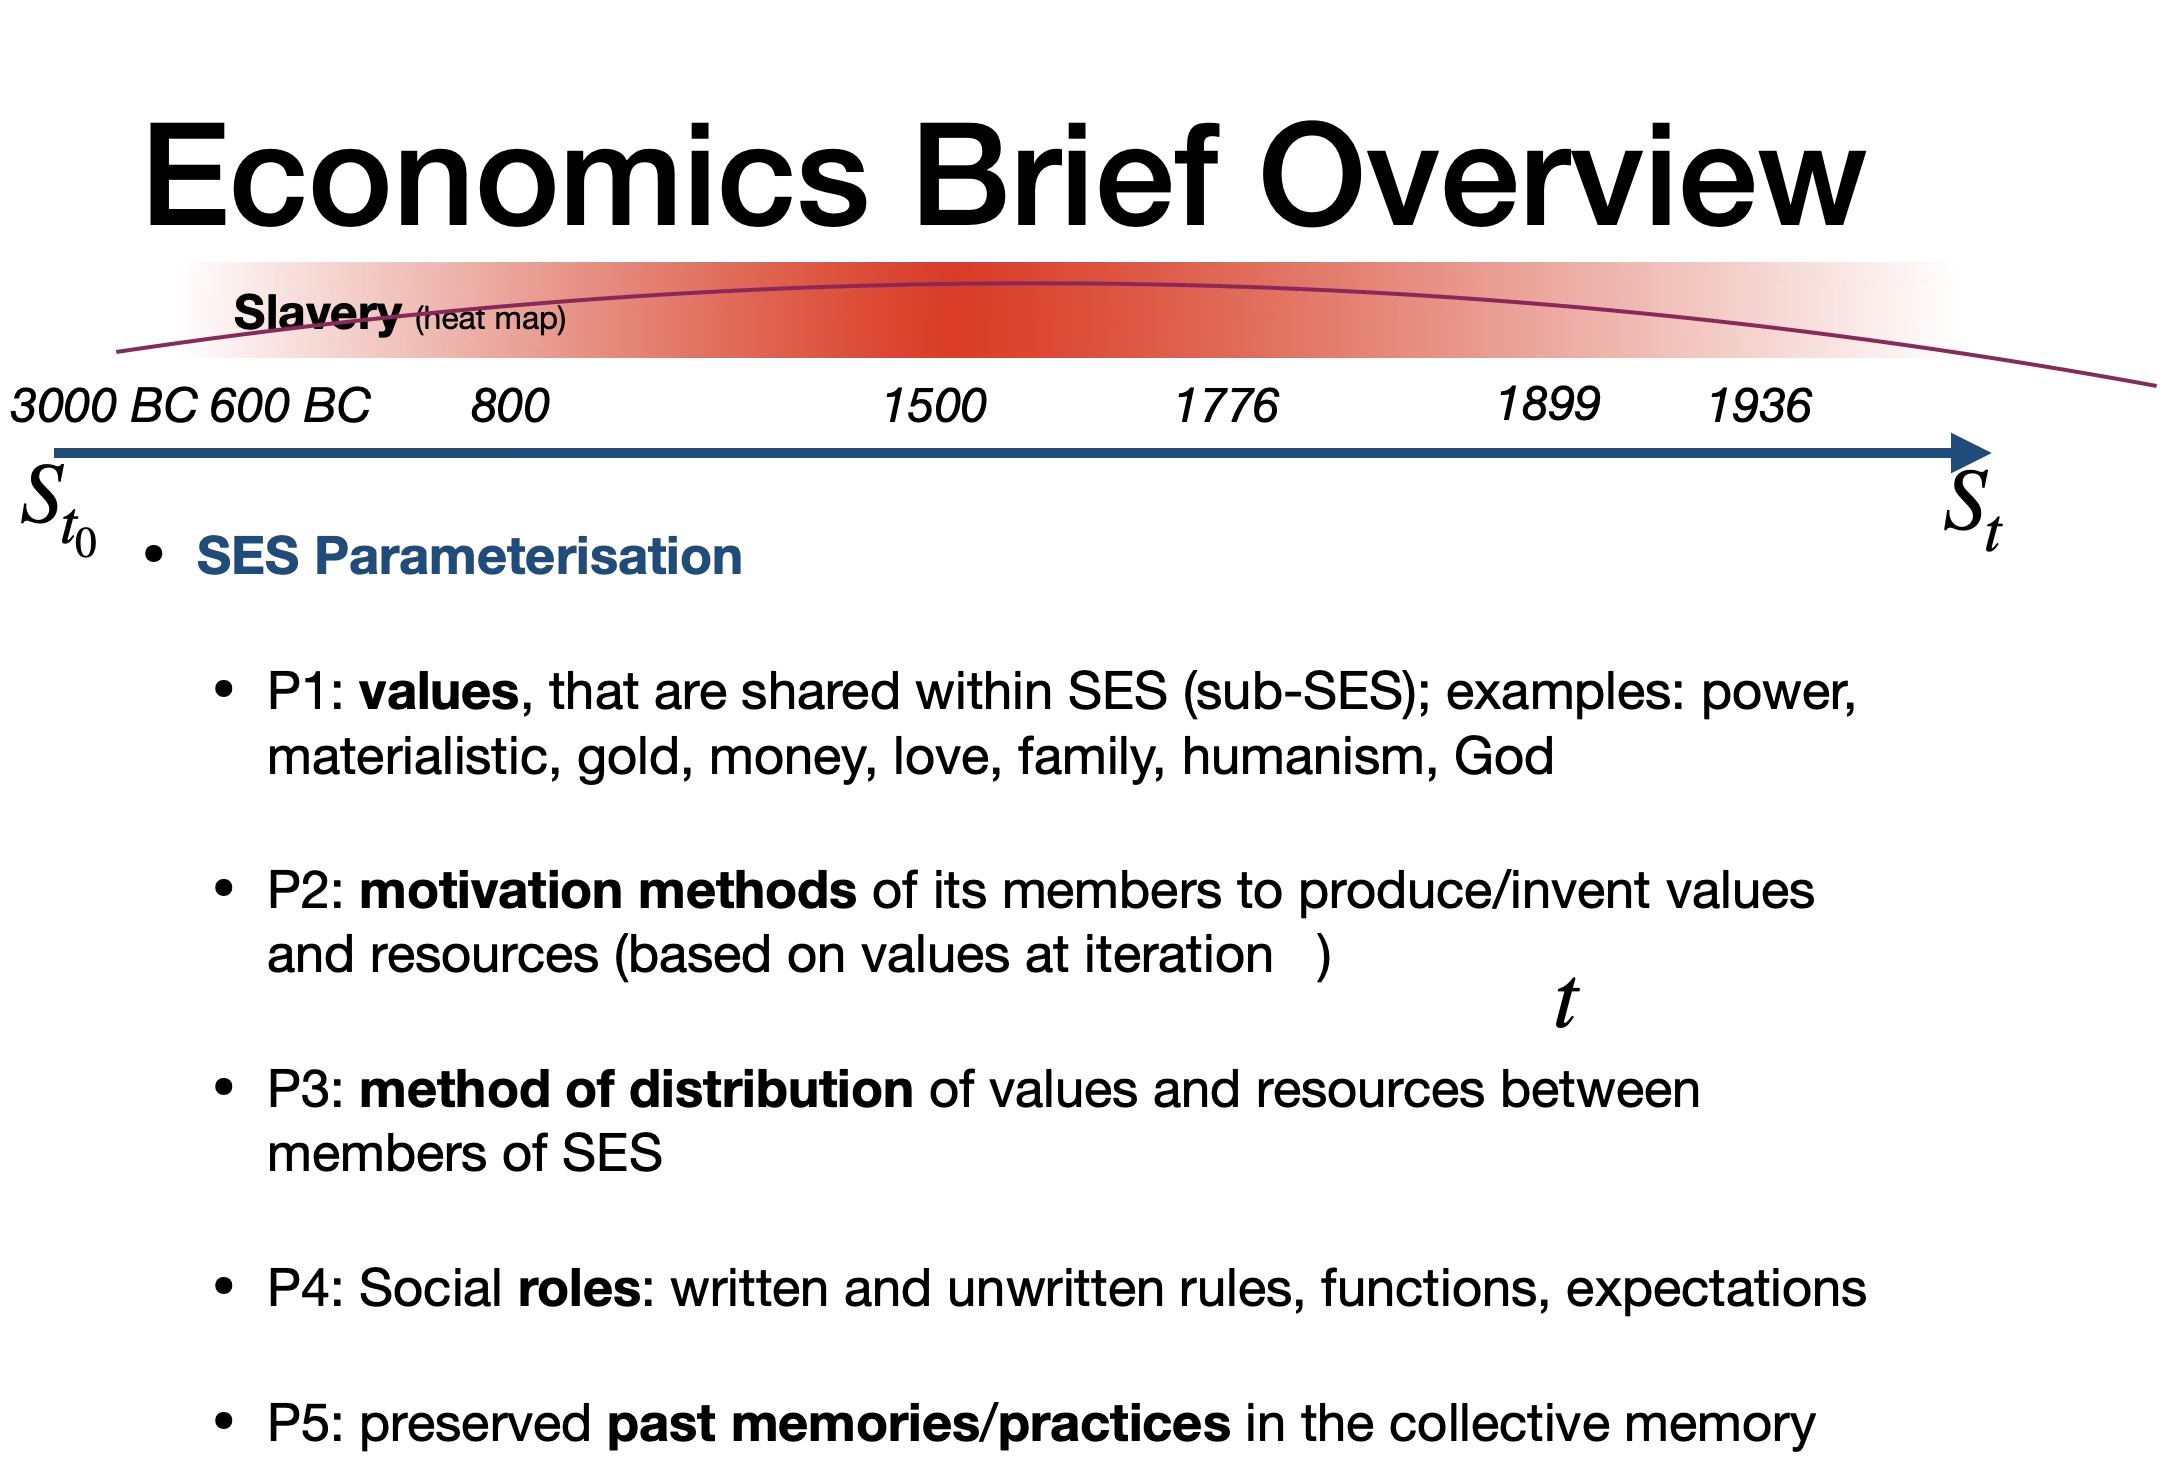
\includegraphics[width=0.9\textwidth]{fig/ses_parameterisation.png}
    \caption{\textbf{SES Parameterization Overview}: Summary of the five key parameters (П1-П5) that characterize any socio-economic system. These parameters are not independent—they interact to create the overall "shape" of the consciousness manifold.}
    \label{fig:ses_params}
\end{figure}

\begin{figure}[H]
    \centering
    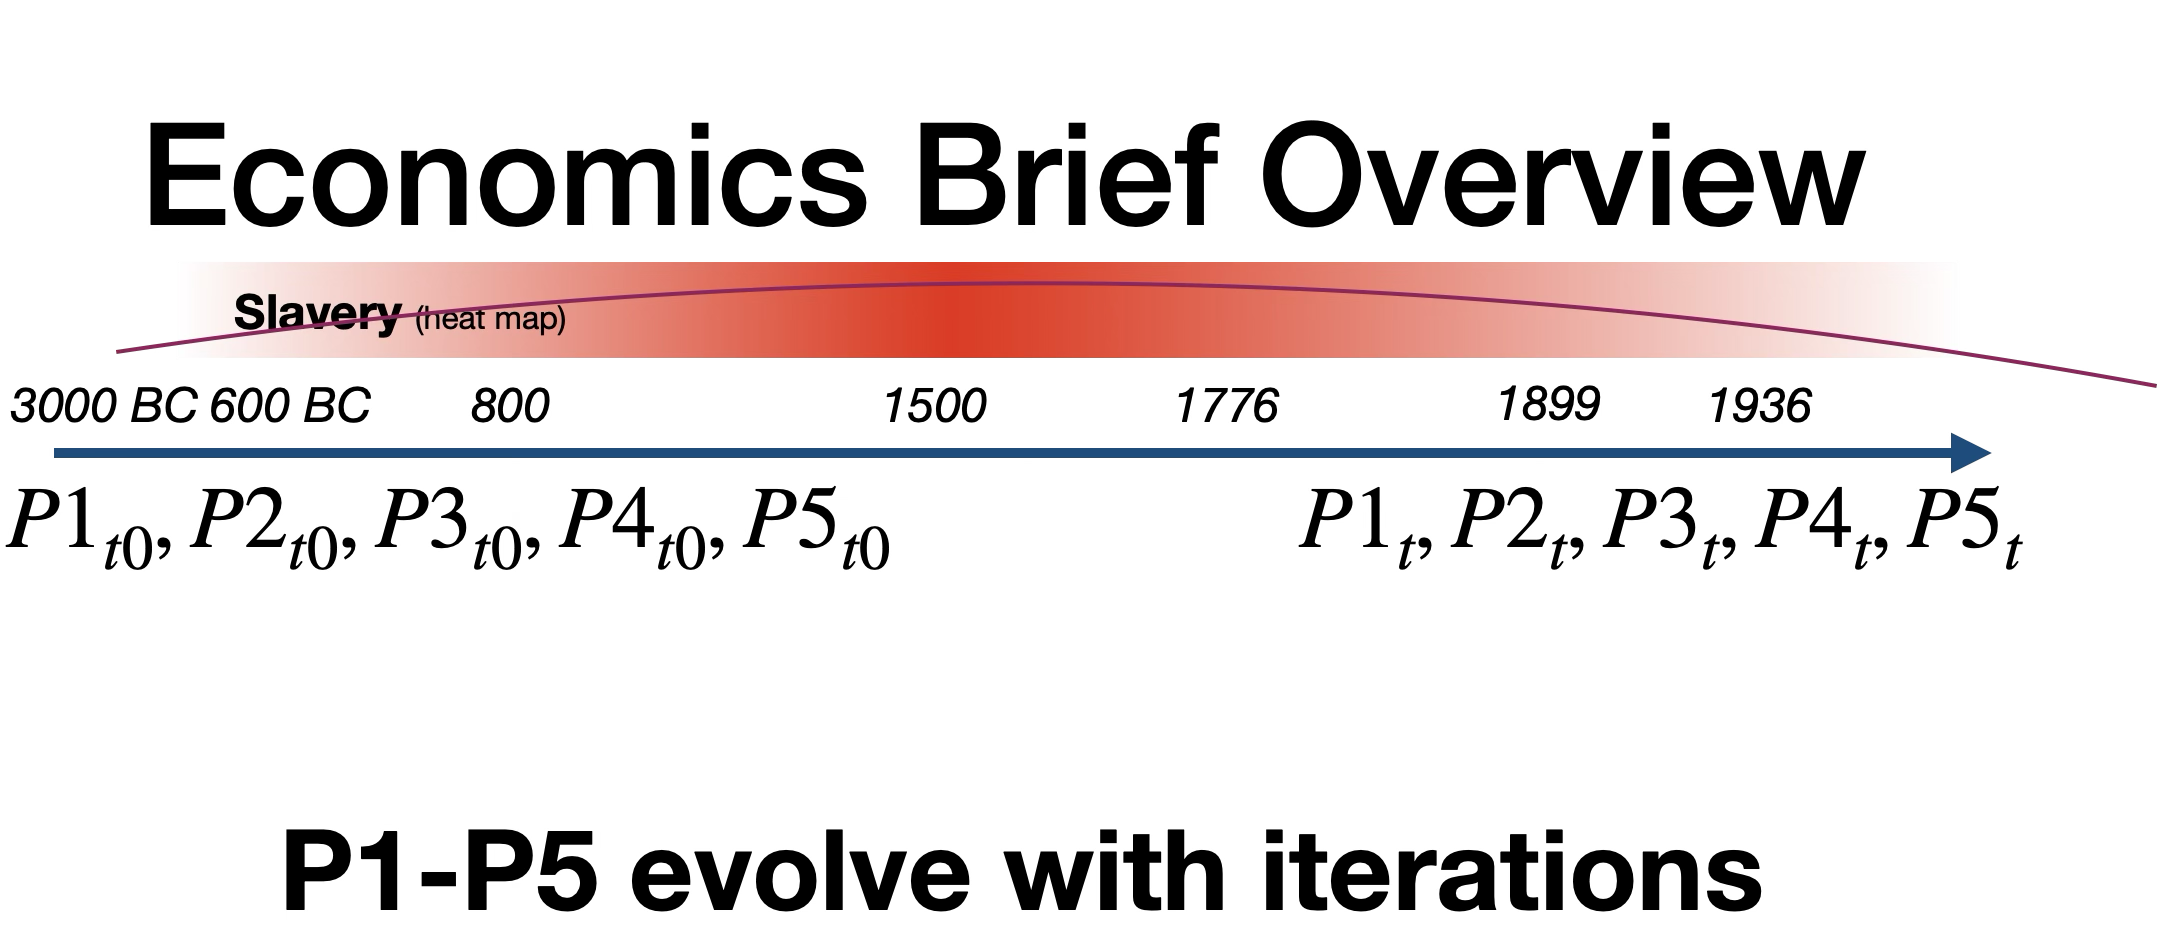
\includegraphics[width=0.9\textwidth]{fig/ses_params_evolution.png}
    \caption{\textbf{Historical Evolution of SES Parameters}: How П1-П5 have changed over time, particularly the sharp divergence since the 1970s-1980s with the rise of neoliberalism, financialization, and digitization. Note how all five parameters trend toward configurations that increase \SYSTEM{} power.}
    \label{fig:ses_evolution}
\end{figure}

\subsection{The Digitization Accelerator: How Modern Technology Amplifies \SYSTEM{}}

One of the most critical developments of the 21st century is the \textit{digitization} of economic and social life. While often celebrated as "progress," digitization has become a powerful accelerant of \SYSTEM{} dynamics, particularly wealth concentration and \betaDehum{}.

\subsubsection{Mechanism: Inserting into Transaction Chains}

Traditional economy: Person A exchanges value with Person B directly (or through simple intermediary).

Digital economy: Platforms insert themselves into every transaction:
\begin{itemize}
\item Ride-sharing: Driver ↔ Platform ↔ Rider (platform extracts 20-30\%)
\item E-commerce: Seller ↔ Platform ↔ Buyer (platform extracts fees + data)
\item Social interaction: Human ↔ Algorithm ↔ Human (platform extracts attention → ad revenue)
\end{itemize}

\textbf{The Pumping Effect:} Like a one-way valve, each digital intermediation extracts value upward toward platform owners while providing minimal direct value to participants. Crucially, once a platform achieves dominance (network effects), it becomes nearly impossible to bypass.

\begin{figure}[H]
    \centering
    \begin{subfigure}[b]{0.48\textwidth}
        \includegraphics[width=\textwidth]{fig/digitization_and_inequality.png}
        \caption{Digitization \& AI impact on inequality through modern economic structures}
    \end{subfigure}
    \hfill
    \begin{subfigure}[b]{0.48\textwidth}
        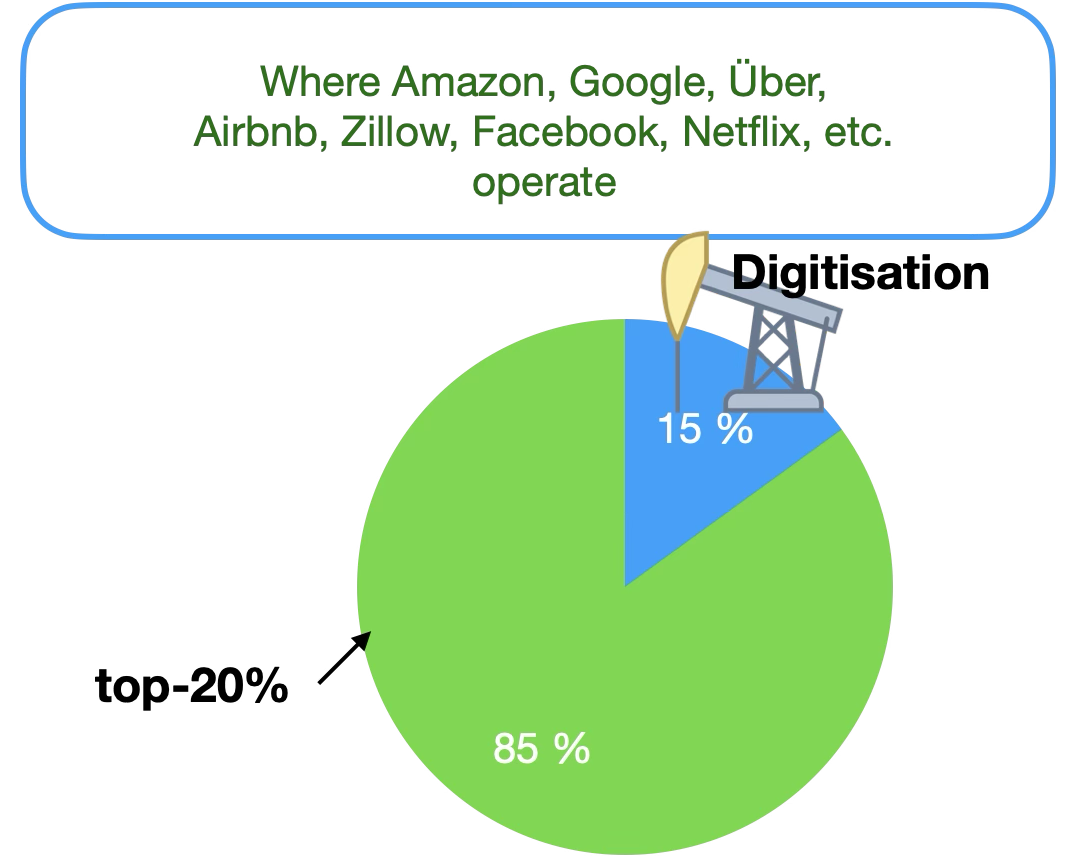
\includegraphics[width=\textwidth]{fig/digitization_and_inequality_pumping_value.png}
        \caption{Value-pumping metaphor: digital platforms as extractive mechanisms}
    \end{subfigure}
    \caption{\textbf{The Digital Acceleration of Inequality}: How digitization and AI serve as "pumps" that accelerate wealth concentration by inserting into transaction chains between humans.}
    \label{fig:digitization}
\end{figure}

\begin{figure}[H]
    \centering
    \begin{subfigure}[b]{0.32\textwidth}
        \includegraphics[width=\textwidth]{fig/digitization_and_inequality_pumping_value_example_part1.png}
        \caption{Part 1: Direct transaction}
    \end{subfigure}
    \hfill
    \begin{subfigure}[b]{0.32\textwidth}
        \includegraphics[width=\textwidth]{fig/digitization_and_inequality_pumping_value_example_part2.png}
        \caption{Part 2: Platform insertion}
    \end{subfigure}
    \hfill
    \begin{subfigure}[b]{0.32\textwidth}
        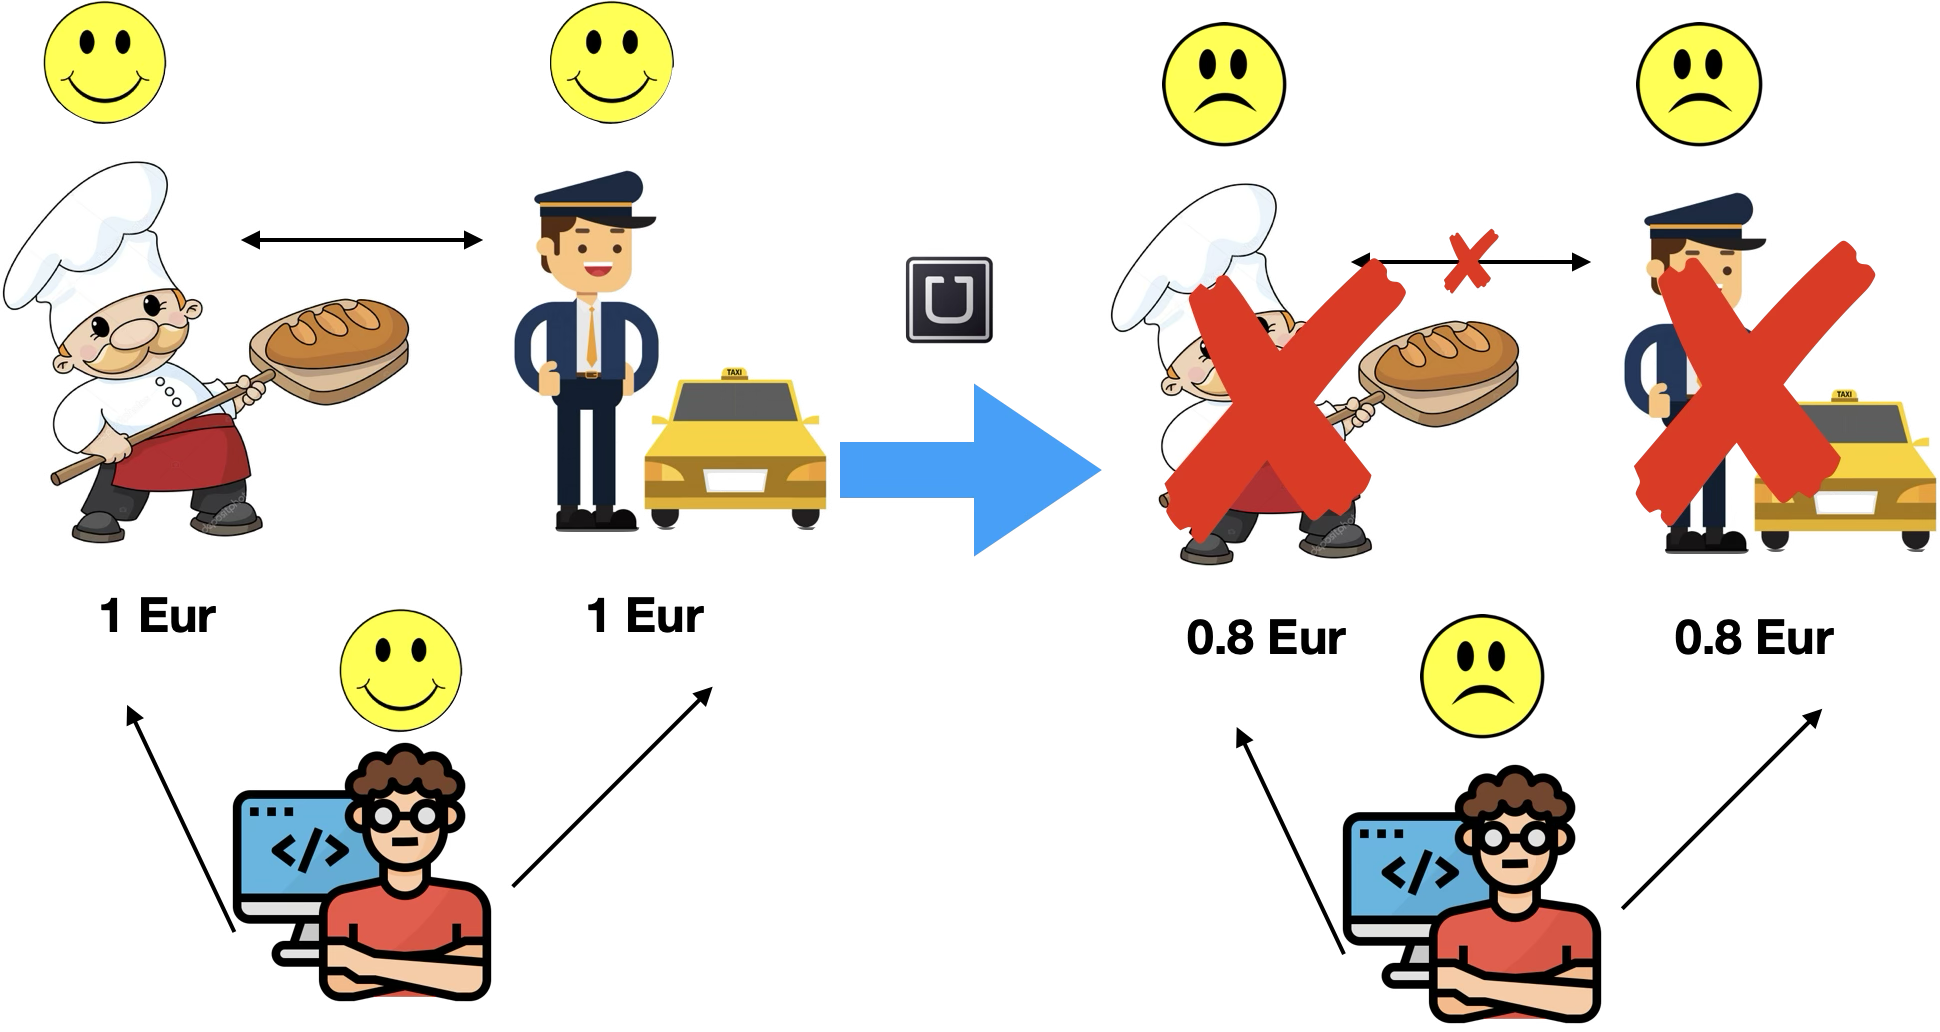
\includegraphics[width=\textwidth]{fig/digitization_and_inequality_pumping_value_example_part3.png}
        \caption{Part 3: Cumulative extraction}
    \end{subfigure}
    \caption{\textbf{Detailed Example of Value Extraction}: Three-stage illustration showing how platform capitalism systematically extracts value from human interactions.}
    \label{fig:extraction_example}
\end{figure}

\subsubsection{Impact on \SES{} Parameters}

Digitization systematically worsens all five parameters:
\begin{itemize}
\item \textbf{П1 (Incentive)}: Platforms optimize for engagement (addiction), not well-being
\item \textbf{П2 (Resources)}: Accelerates wealth concentration (tech billionaires become trillionaires)
\item \textbf{П3 (Information)}: Algorithmic control over perception unprecedented in human history
\item \textbf{П4 (Transparency)}: Algorithms are black boxes; corporate secrecy protects mechanisms
\item \textbf{П5 (Temporal)}: Instant gratification culture; "move fast and break things"
\end{itemize}

\begin{figure}[H]
    \centering
    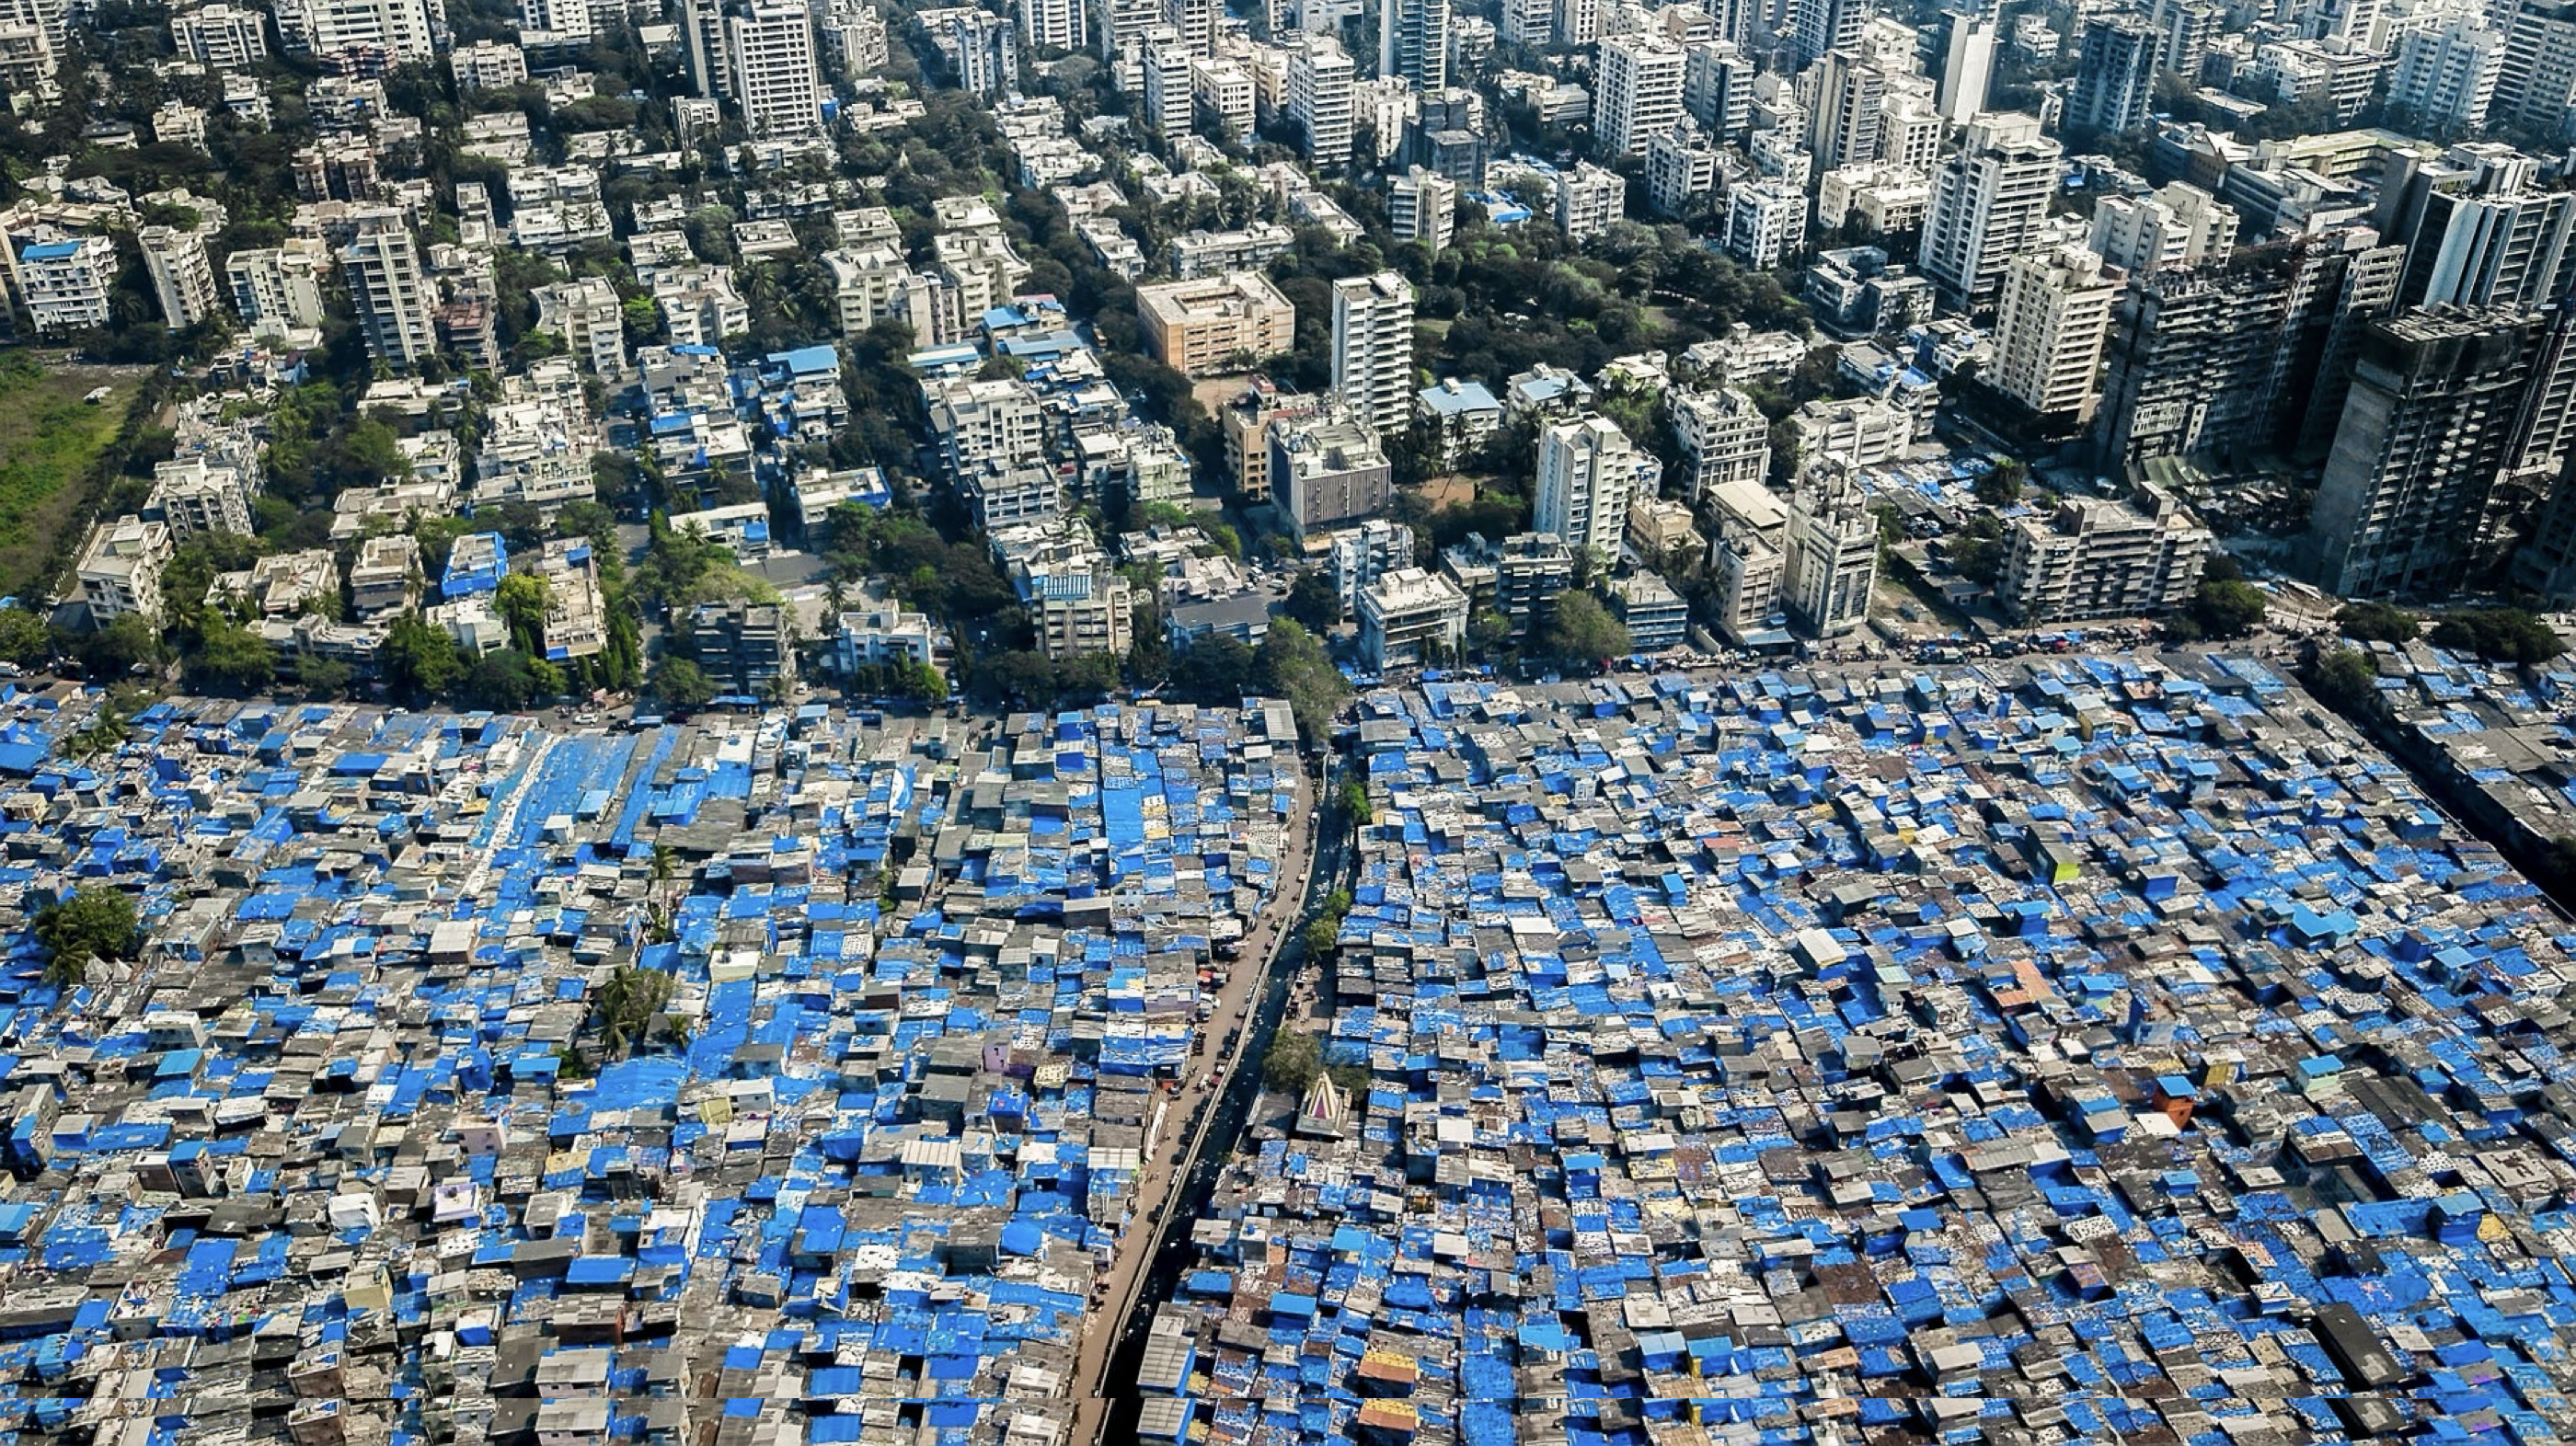
\includegraphics[width=0.65\textwidth]{fig/inequality_illustration.png}
    \caption{\textbf{Visual Metaphor for Inequality}: The material reality of extreme wealth concentration—luxury estates next to informal settlements, separated by a wall. This is not just economic disparity but \textit{ontological} disparity in lived reality.}
    \label{fig:inequality_visual}
\end{figure}

\subsection{Money: Not Just Medium of Exchange, but Instrument of Control}

To understand \SYSTEM{} fully, we must re-examine what money \textit{actually is} in modern systems.

\begin{definition}[Money — Operational Definition]
\label{def:money}
Money serves multiple functions:
\begin{enumerate}
\item \textbf{Medium of Exchange}: Facilitates transactions
\item \textbf{Store of Value}: Preserves purchasing power over time
\item \textbf{Unit of Account}: Measures relative worth
\item \textbf{Instrument of Direction}: Allocates human attention and effort
\item \textbf{Issuer of Permission}: Gatekeeps access to resources and opportunities
\item \textbf{Instrument of Control}: Shapes behavior through reward/punishment
\end{enumerate}

Functions 4-6 are often ignored in economics textbooks but are central to \SYSTEM{} dynamics.
\end{definition}

\begin{example}[The Dollar and Gold Decoupling]
In 1971, President Nixon ended the Bretton Woods system, severing the dollar's tie to gold. This seemingly technical change had profound implications:

\textbf{Before:} Money supply constrained by physical gold reserves \\
\textbf{After:} Money supply controlled by central bank policy (effectively, printing at will)

\textbf{Consequence:} Those who control money creation (central banks, commercial banks via fractional reserve lending) control vast flows of human energy and attention. Inflation disproportionately harms those without assets (wage earners) while benefiting asset holders (capital owners).

\textbf{Geometric interpretation:} The dollar's decoupling from gold removed a "natural constraint" on \CC{} distortions, allowing greater artificial curvature to be introduced through monetary policy.
\end{example}

\begin{figure}[H]
    \centering
    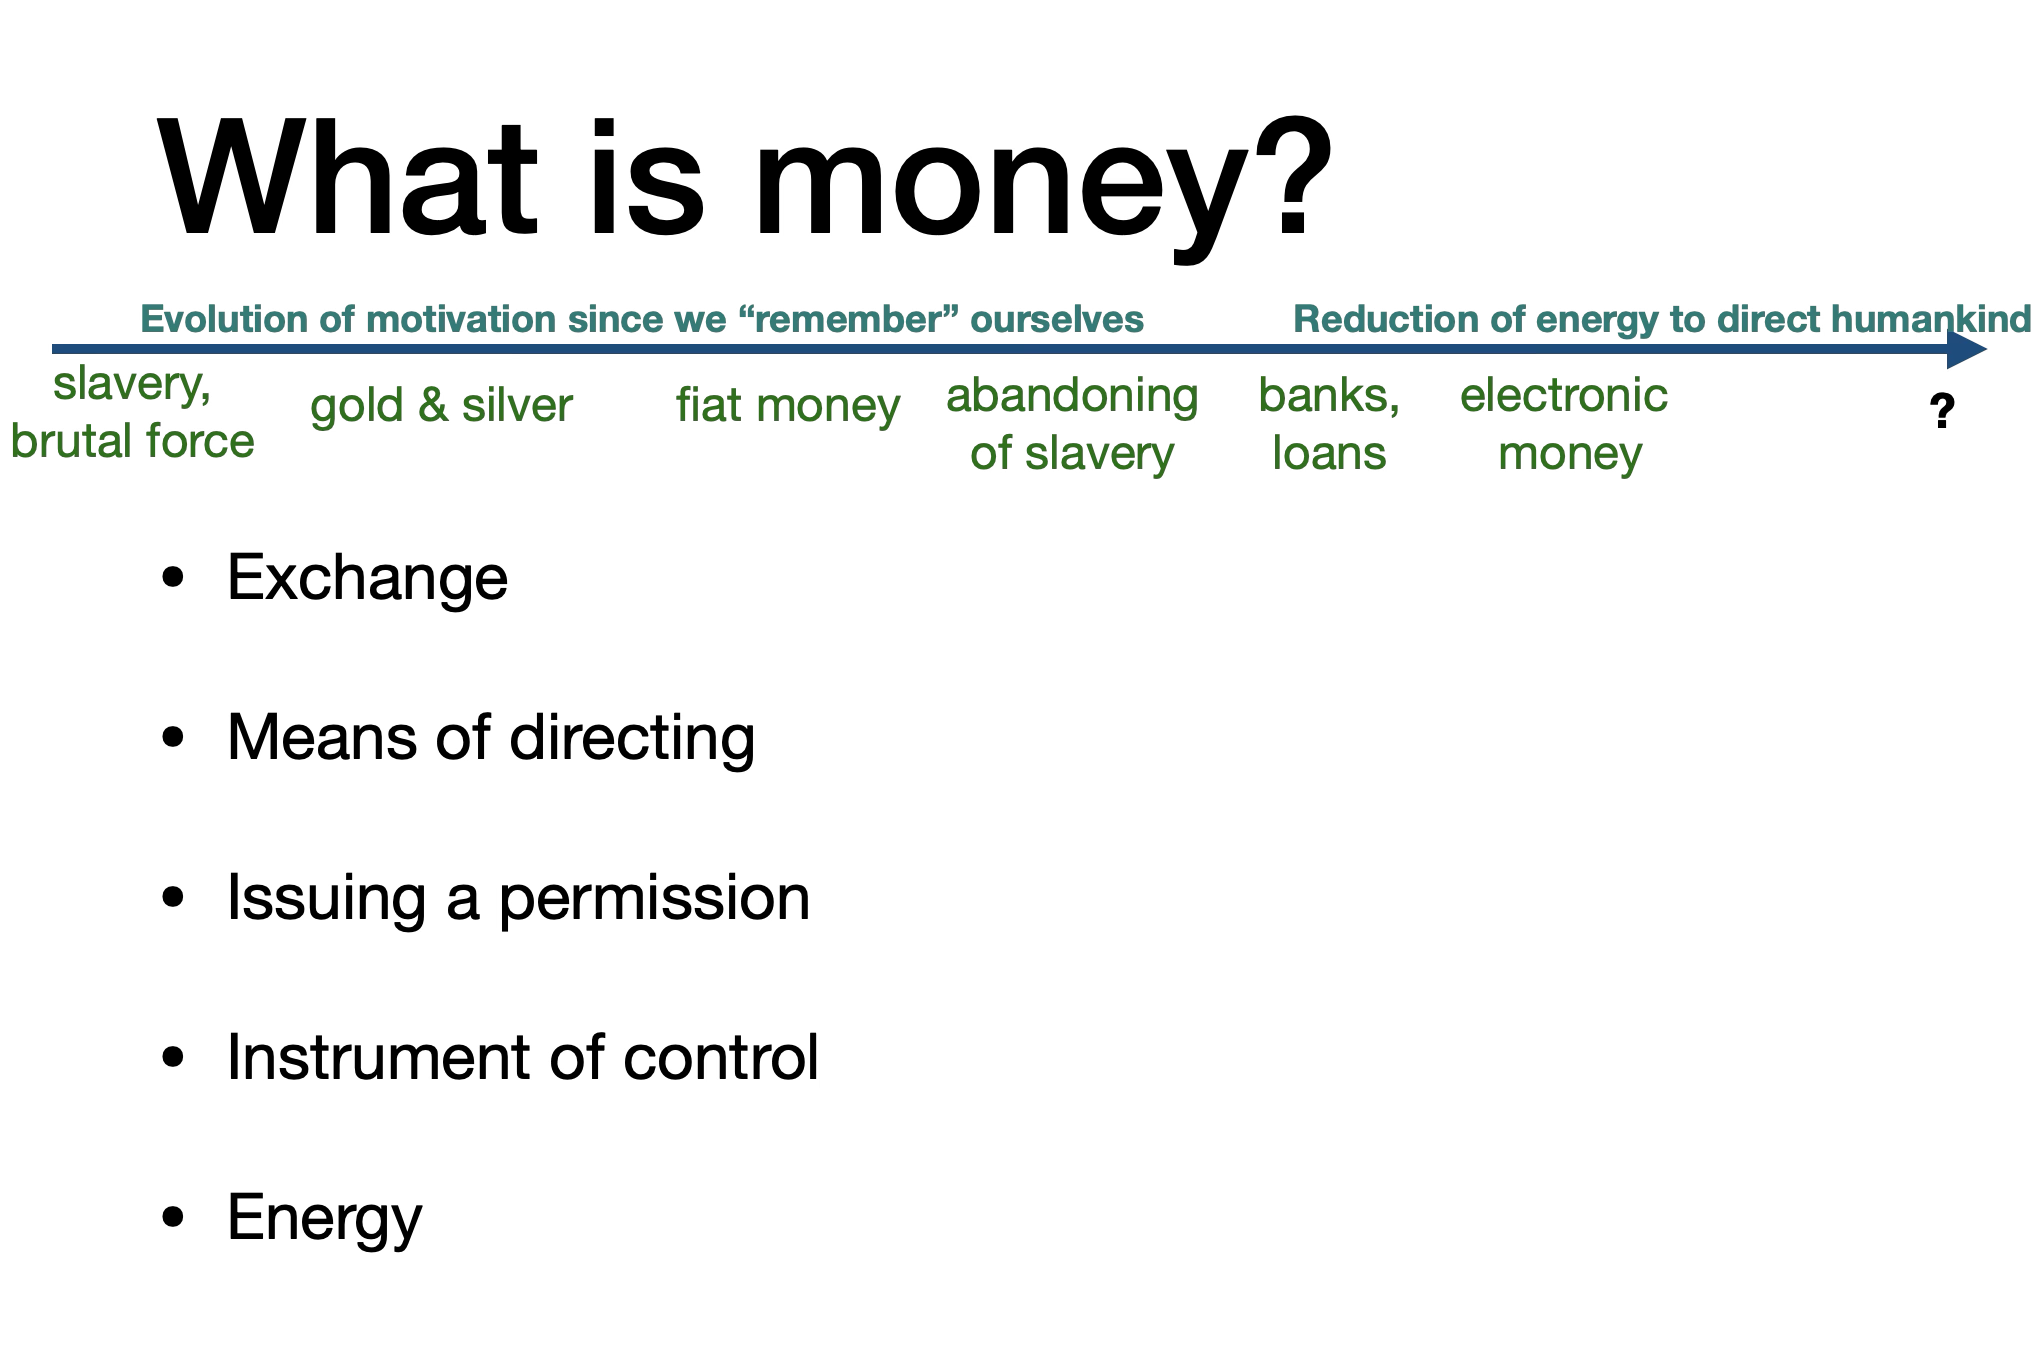
\includegraphics[width=0.55\textwidth]{fig/what_is_money.png}
    \caption{\textbf{What is Money?} (Illustration in Russian, key concepts: Exchange, Means of Directing, Issuing Permission, Control Instrument, Energy). Money is not a neutral tool but a technology that shapes consciousness and social relations.}
    \label{fig:what_is_money}
\end{figure}

% ==========================================
% PART II: SYSTEM MANIFESTATIONS
% ==========================================

\section{Part II: \SYSTEM{} in Action — Case Studies and Mechanisms}

Having established the theoretical framework, we now examine how \SYSTEM{} manifests in concrete historical and contemporary phenomena.

\subsection{The Stanford Prison Experiment: \betaDehum{} in Laboratory Conditions}

\begin{example}[Zimbardo's SPE, 1971]
\cite{spe} In this famous experiment, psychologically healthy college students were randomly assigned to "prisoner" or "guard" roles in a simulated prison. Within days:

\begin{itemize}
\item Guards exhibited sadistic behavior, humiliating and psychologically abusing prisoners
\item Prisoners became passive, depressed, and dehumanized
\item Even the researchers lost objectivity, becoming absorbed in the system
\end{itemize}

\textbf{Key Insight:} The \textit{structure} (roles, power dynamics, environmental cues) induced \betaDehum{} in otherwise good people. This demonstrates \textbf{Axiom \ref{ax:ses_embedding}}: socio-economic structures shape unconscious behavior.

\textbf{Geometric interpretation:} The experimental setup created a local distortion in \CC{} (a "prison attractor basin"). Once inside, geodesics bent toward dehumanizing behaviors—it became the path of least resistance.
\end{example}

\begin{figure}[H]
    \centering
    \includegraphics[width=0.75\textwidth]{fig/prison_experiment_illustration_delta_dehumanisation_dynamics.png}
    \caption{\textbf{Prison Experiment and \betaDehum{} Dynamics}: Illustration showing how quickly systemic roles induce dehumanization. The \betaDehum{} parameter $\beta$ increases rapidly under structural pressure, independent of individual "goodness."}
    \label{fig:prison_experiment}
\end{figure}

\subsection{Israel and Collective Trauma: When National Identity Becomes \SYSTEM{} Hostage}

\textit{Note: This analysis is not anti-Semitic or anti-Israeli; it is a compassionate examination of how trauma perpetuates harmful patterns. The goal is healing, not blame.}

\begin{example}[Post-Holocaust Trauma and Israeli Policy]
The Holocaust represents one of history's most profound collective traumas. The State of Israel was founded (1948) in its immediate aftermath, carrying this trauma as a core element of national identity.

\textbf{Trauma → \SYSTEM{} feedback loop:}
\begin{enumerate}
\item Trauma creates \textit{existential fear} ("never again")
\item Fear demands \textit{absolute security} (maximalist military doctrine)
\item Absolute security requires \textit{viewing neighbors as threats} (\betaDehum{} of Palestinians)
\item Dehumanization enables \textit{disproportionate violence} (Gaza, West Bank policies)
\item Violence generates \textit{more trauma} (for both Israelis and Palestinians)
\item Cycle reinforces itself; questioning it becomes "existential threat" to national identity
\end{enumerate}

\textbf{The "Hostage" Dynamic:} Most Israelis are \textit{not} consciously choosing cruelty. They are operating within a \SYSTEM{}-generated attractor basin where:
\begin{itemize}
\item Education emphasizes victimhood narrative
\item Military service is mandatory (normalizing violence)
\item Media presents Palestinians as existential threat
\item Dissent is labeled treason
\end{itemize}

\textbf{Geometric interpretation:} Post-Holocaust trauma introduced extreme curvature into the Israeli consciousness manifold. Geodesics leading toward peace require "uphill" traversal (high activation energy), while paths toward militarism are "downhill" (locally stable, even if globally destructive).

\textbf{Path to healing:} Requires (1) acknowledging trauma without letting it justify harm, (2) extending empathy to "the other," (3) structural reforms (e.g., truth and reconciliation, economic integration). This is precisely what S.V.E. protocols aim to facilitate.
\end{example}

\subsection{Education: Manufacturing Compliant Minds}

Russell's epigraph captures a disturbing truth: modern education systems often prioritize conformity over critical thinking.

\begin{proposition}[\SYSTEM{} and Education]
\label{prop:education}
Educational institutions under \SYSTEM{} tend to:
\begin{enumerate}
\item Reward memorization and obedience over questioning and creativity
\item Suppress "uncomfortable" topics (history of imperialism, class struggle, structural inequality)
\item Emphasize nationalist narratives and emotional loyalty
\item Channel students into economic roles that serve \SYSTEM{} (corporate drones, not philosophers)
\end{enumerate}

\textbf{Mechanism:} Those who control resources (capitalists, militarists, religious institutions) exert influence over curricula. They fund universities, sit on boards, shape research priorities. The result is "intellectual monoculture" aligned with \SYSTEM{} perpetuation.
\end{proposition}

\begin{remark}
This is not absolute—pockets of resistance exist (critical pedagogy, free universities, S.V.E. itself). But the \textit{dominant tendency} is toward instrumentalization of education.
\end{remark}

\subsection{Social Media: The Attention Economy as \SYSTEM{} Infrastructure}

Social media platforms represent one of the most sophisticated \SYSTEM{} tools ever created.

\begin{proposition}[Social Media and Consciousness Colonization]
\label{prop:social_media}
Platforms like Facebook, Instagram, TikTok, Twitter/X operate by:
\begin{enumerate}
\item \textbf{Hijacking dopamine systems}: Infinite scroll, likes, notifications → addiction
\item \textbf{Algorithmic curation}: Showing content that maximizes "engagement" (often outrage, tribalism)
\item \textbf{Fragmenting attention}: Reducing capacity for sustained thought
\item \textbf{Monetizing intimacy}: Transforming relationships into data and ad targeting
\item \textbf{Amplifying \betaDehum{}}: Anonymous mobs, dehumanizing rhetoric, echo chambers
\end{enumerate}

\textbf{The Zuckerberg Paradox:} Mark Zuckerberg's famous post after paternity leave showed a closet full of identical gray T-shirts, with the caption "What should I wear?" This symbolizes a man who values simplicity, focus, and substance in his own life while building a platform that does the opposite for billions—promotes vanity, distraction, and superficiality.

\textbf{The Question (not judgment):} How can someone with such values create tools that undermine those very values? The answer: He is operating within \SYSTEM{}, optimizing for metrics (user growth, ad revenue) without full awareness of the downstream consequences. He is both architect and hostage.
\end{proposition}

\begin{figure}[H]
    \centering
    
\includegraphics[width=0.7\textwidth]{fig/socialmedia_illustration_pr-pretending_vs_being.png}
    \caption{\textbf{Social Media: Pretending vs. Being}: Illustration of how social media platforms incentivize performance and impression management over authentic self-expression, accelerating \betaDehum{} by reducing people to curated brands.}
    \label{fig:social_media}
\end{figure}

\begin{figure}[H]
    \centering
    \includegraphics[width=0.8\textwidth]{fig/mark_zuckerberg_inconsistency_goal_reality.png}
    \caption{\textbf{The Zuckerberg Inconsistency}: Zuckerberg's personal aesthetic (minimalist, focused on substance) versus the platform he created (maximalist, focused on appearance and engagement metrics). This is not hypocrisy but \textit{unconscious participation in \SYSTEM{}}.}
    \label{fig:zuckerberg}
\end{figure}

\begin{figure}[H]
    \centering
    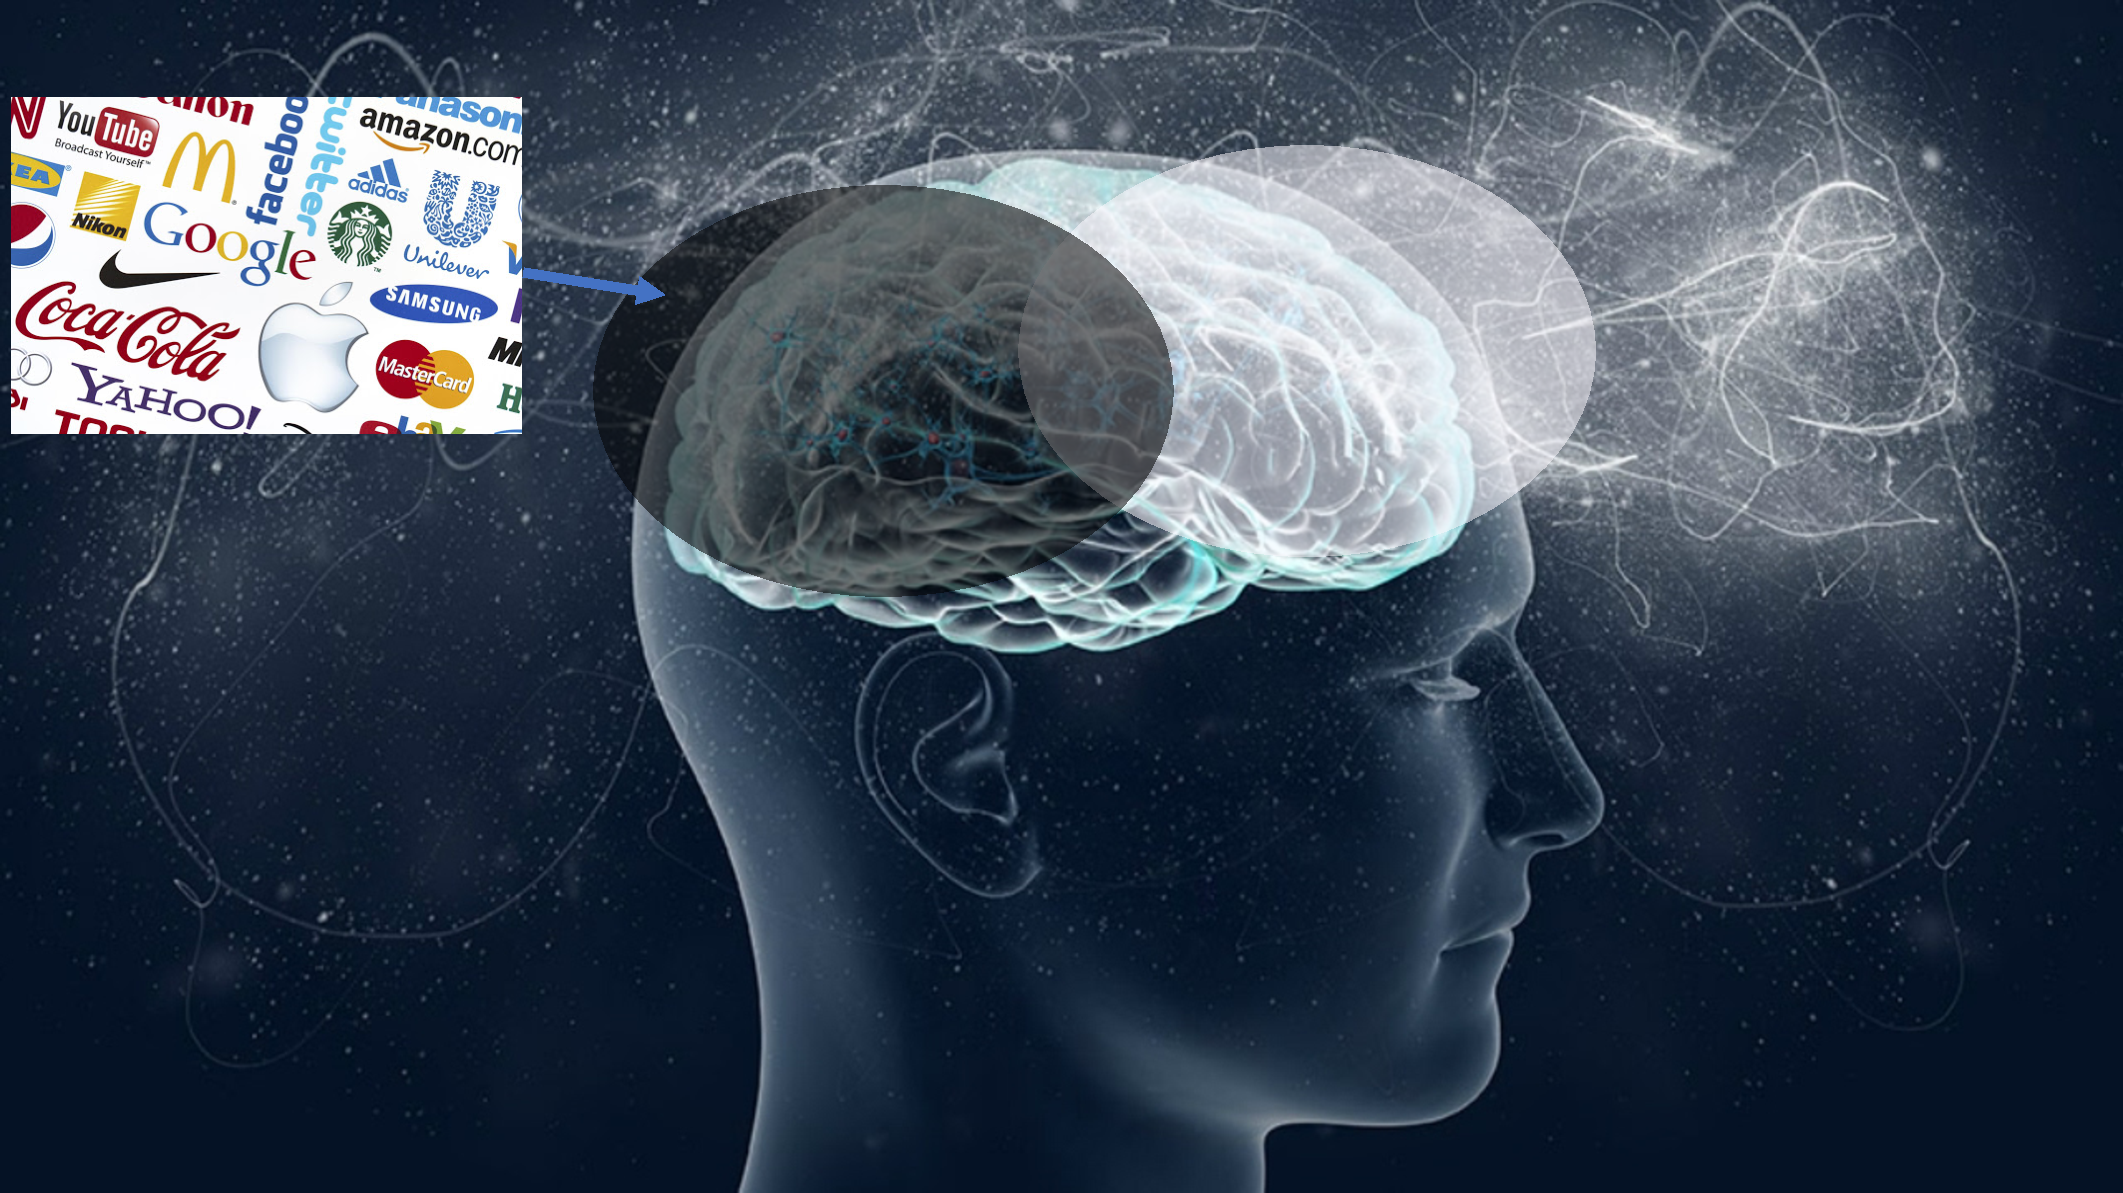
\includegraphics[width=0.85\textwidth]{fig/attention_economy_brands_as_real_estates_in_conciousness_space.pdf}
    \caption{\textbf{Attention Economy}: Brands and platforms as "real estate" in consciousness space. Just as physical real estate requires ongoing rent payments, psychological real estate (brand awareness, habitual app usage) extracts ongoing attention-rent from humans. The consciousness manifold becomes colonized.}
    \label{fig:attention_economy}
\end{figure}

\subsection{Satanic Chess: When Elites Play Games with Human Lives}

\textit{Note: "Satanic" here is metaphorical, not theological—referring to adversarial, zero-sum, dehumanizing strategy.}

The term "Satanic Chess" comes from strategic thinking traditions (Pereslegin \cite{pereslegin_summa}, Machiavelli \cite{machiavelli_prince}, Sun Tzu \cite{sun_tzu_art_of_war}) where geopolitical actors treat human beings as pieces on a board.

\begin{example}[Iraq War (2003) as Satanic Chess]
\textbf{Official narrative:} Liberate Iraq from Saddam Hussein, find WMDs, spread democracy.

\textbf{Revealed reality:} No WMDs found. True motives: (1) Control oil resources, (2) Test military technologies, (3) Enrich defense contractors, (4) Establish regional hegemony.

\textbf{Human cost:} Estimates range from 200,000 to 1 million Iraqi deaths, millions displaced, country destabilized for decades.

\textbf{\SYSTEM{} Analysis:} Decision-makers (Bush, Cheney, Rumsfeld, etc.) were not comic-book villains. They operated within a system where:
\begin{itemize}
\item \textbf{П1 (Incentive)}: Personal and institutional rewards aligned with war (defense industry profits, political capital)
\item \textbf{П3 (Information)}: Intelligence agencies provided justifying narratives; media amplified propaganda
\item \textbf{П4 (Transparency)}: Decisions made in classified contexts; dissent suppressed
\item \textbf{\betaDehum{}}: Iraqi lives counted less than American "strategic interests"
\end{itemize}

\textbf{The Hostage Aspect:} Many in the "elite" class (politicians, military brass, think-tank analysts) are themselves products of systems that reward ruthlessness and punish compassion. A U.S. President who prioritizes Iraqi lives over "national interest" would be ousted. The system selects for those willing to play the game.
\end{example}

\begin{figure}[H]
    \centering
    
\includegraphics[width=0.8\textwidth]{fig/delta_dehumanisation_self_stimulating_circle.png}
    \caption{\textbf{\betaDehum{} Self-Stimulating Cycle}: Once initiated, dehumanization creates feedback loops—violence breeds trauma, trauma breeds fear, fear breeds more dehumanization. Breaking the cycle requires external intervention (awareness, structural change).}
    \label{fig:beta_dehum_cycle}
\end{figure}

\subsection{"Dark Arts" Operations: Historical Examples of Conscious \SYSTEM{} Exploitation}

While \SYSTEM{} often operates unconsciously, there are cases where powerful actors \textit{deliberately} exploit its dynamics for strategic advantage. We call these "Dark Arts" operations—not because they're supernatural, but because they manipulate from shadow, hiding true motives.

\begin{example}[Tuskegee Syphilis Study (1932-1972)]
U.S. Public Health Service studied syphilis progression in African American men by \textit{withholding treatment} (even after penicillin became available). Participants were told they were receiving "free healthcare."

\textbf{\betaDehum{} mechanism:} Racist ideology allowed researchers to view Black men as "expendable research subjects" rather than humans deserving dignity and care.

\textbf{\SYSTEM{} enabler:} Institutional structures (medical hierarchy, racial segregation, scientific authority) provided cover for decades.
\end{example}

\begin{example}[Guatemala Syphilis Experiments (1946-1948)]
U.S. researchers deliberately infected Guatemalan prisoners, psychiatric patients, and sex workers with syphilis to study disease progression. No informed consent.

\textbf{Parallel:} Similar \betaDehum{} logic—Guatemalans viewed as "less human," therefore ethically permissible to harm for scientific gain.
\end{example}

\begin{example}[Operation Paperclip (1945-)]
U.S. government secretly recruited Nazi scientists (including war criminals involved in human experimentation) to work on American military projects.

\textbf{\SYSTEM{} logic:} "Strategic value" outweighed ethical concerns. \betaDehum{} of Nazi victims ("that was the past"), prioritization of Cold War competition.
\end{example}

\textbf{Pattern Recognition:} These are not isolated cases but manifestations of a systemic tendency: When \SYSTEM{} dynamics dominate (П1 misaligned, П4 opacity), even institutions nominally dedicated to human welfare (medicine, science) can commit atrocities.

\subsection{The "Parent-Child" Metaphor for 1\% and 99\%}

One of the most provocative ways to understand the 1\%/99\% dynamic is through a family metaphor.

\begin{figure}[H]
    \centering
    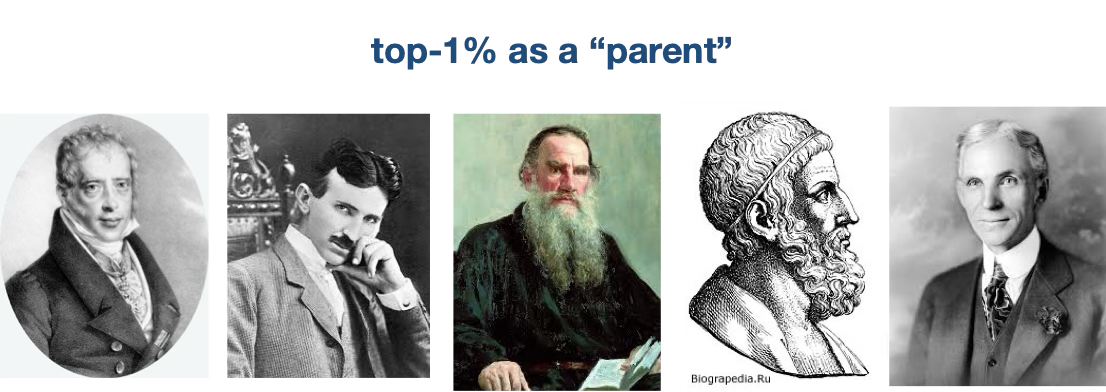
\includegraphics[width=0.75\textwidth]{fig/top1percent_as_Parent_for_Humanity.png}
    \caption{\textbf{Top 1\% as "Parents" for Humanity}: Illustration showing figures like Einstein, Tesla, Gates, Musk positioned as "parental" figures. The question: Are they good parents? Do they guide humanity toward flourishing, or do they impose their own agendas? This is not to deify or demonize individuals but to examine the \textit{structural role} wealth and power confer.}
    \label{fig:top1percent_parent}
\end{figure}

\begin{proposition}[The Parent-Child Dynamic]
\label{prop:parent_child}
In current \SES{}, the top 1\% (particularly top 0.01\%) function as de facto "parents" for humanity:
\begin{itemize}
\item They control resources (wealth, media, technology)
\item They shape narratives (what is "possible," "desirable," "normal")
\item They make decisions affecting billions (e.g., Zuckerberg's algorithm changes, Musk's Twitter policies, Bezos's labor practices)
\end{itemize}

\textbf{The Question:} Are they \textit{good} parents? Do they prioritize humanity's well-being (children's flourishing), or their own interests (maintaining wealth/power)?

\textbf{The Answer (from \SYSTEM{} perspective):} Most are \textit{not consciously malicious} but are \textit{trapped in a system} that rewards short-term extraction over long-term stewardship. They are "parents" who never asked for the role and have no training for it. Moreover, \SYSTEM{} selects for sociopathic tendencies (ruthlessness is rewarded in competition for dominance).

\textbf{The Hope:} Just as dysfunctional parenting patterns can be healed through awareness and therapy, \SYSTEM{} patterns can be healed through awareness and structural reform.
\end{proposition}

% ==========================================
% PART III: GEOMETRIC & PSYCHOLOGICAL DEEP DIVE
% ==========================================

\section{Part III: The Geometry of the Fall — Jung, Plato, and the Consciousness Manifold}

\subsection{Jung's Collective Unconscious as \SYSTEM{} Substrate}

Carl Jung's concept of the collective unconscious \cite{jung_collective_unconscious} provides the psychological foundation for \SYSTEM{}.

\begin{definition}[Collective Unconscious \CU{}]
\label{def:collective_unconscious}
The \textbf{collective unconscious} is the deepest layer of the psyche, shared across humanity, containing:
\begin{itemize}
\item \textbf{Archetypes}: Universal patterns (hero, shadow, trickster, mother, etc.)
\item \textbf{Instincts}: Evolved behavioral dispositions (survival, reproduction, social bonding)
\item \textbf{Trauma imprints}: Collective memory of suffering (wars, famines, oppression)
\end{itemize}

Unlike the personal unconscious (individual repressions), \CU{} is \textit{inherited} and \textit{transpersonal}.
\end{definition}

\textbf{S.V.E. Extension:} We propose that \CU{} is not just psychological but is \textit{instantiated in \SES{} structures}. The "invisible hand" (Smith) is the economic manifestation of unconscious collective dynamics (Jung).

\begin{proposition}[Invisible Hand = Collective Unconscious in Economic Form]
\label{prop:invisible_hand_unconscious}
Adam Smith's "invisible hand" \cite{smith1776wealth} is not a metaphor for rational coordination but for \textit{unconscious coordination}—millions of individuals acting on unconscious drives (fear, greed, status-seeking), producing aggregate outcomes no one intended.

\textbf{Implication:} Market outcomes reflect not "rational choice" but the shape of \CU{} as filtered through \SES{} structures. If \CU{} is distorted (by the Fall), market outcomes will be distorted (inequality, exploitation, ecological destruction).
\end{proposition}

\begin{figure}[H]
    \centering
    \includegraphics[width=0.85\textwidth]{fig/main_illustration_invisible_hand_subconciousness.png}
    \caption{\textbf{The Invisible Hand as Collective Unconscious}: Main illustration linking Adam Smith's invisible hand to Jung's collective unconscious. The hand operates below the surface of awareness, shaping economic outcomes through unconscious drives embedded in \SES{} parameters.}
    \label{fig:invisible_hand}
\end{figure}

\subsection{Plato's Cave: The Shadow on the Consciousness Manifold}

Plato's Cave allegory \cite{plato_republic} provides a geometric model of ignorance and enlightenment.

\begin{example}[The Cave Allegory]
\textbf{Setup:} Prisoners chained in a cave, facing a wall. Behind them, a fire casts shadows of objects onto the wall. Prisoners mistake shadows for reality.

\textbf{Liberation:} A prisoner is freed, turns to see the fire and objects, then ascends to the sunlit world outside. The sun represents ultimate truth/goodness.

\textbf{Challenge:} If the freed prisoner returns to tell others, they ridicule him—they prefer familiar shadows to destabilizing truth.
\end{example}

\textbf{S.V.E. Mapping onto \CC{}:}
\begin{itemize}
\item \textbf{Cave}: Shadow region of \CC{} (unconscious)
\item \textbf{Shadows}: Narratives, illusions, appearances generated by \SYSTEM{}
\item \textbf{Fire}: \SES{} structures casting the shadows (economic incentives, media, education)
\item \textbf{Chains}: Psychological attachments, fears, cognitive biases keeping prisoners fixed
\item \textbf{Sunlight outside}: Fully conscious, integrated awareness (alignment with Truth and Love)
\item \textbf{Freed prisoner}: Those who achieve awareness ("osoznannost' — awareness") and attempt to help others
\end{itemize}

\textbf{Geometric Formalization:}
\begin{align}
\text{Let } \CC_{\text{shadow}} &= \text{region of manifold with high curvature (Fall distortions)} \\
\text{Let } \CC_{\text{light}} &= \text{region with minimal curvature (aligned with Truth)} \\
\text{Transition: } \CC_{\text{shadow}} \to \CC_{\text{light}} &\text{ requires energy (overcoming systemic resistance)}
\end{align}

Most humans remain in $\CC_{\text{shadow}}$ not because they're stupid but because:
\begin{enumerate}
\item It's locally stable (familiar, comfortable)
\item Transition requires high activation energy (confronting uncomfortable truths)
\item \SYSTEM{} actively resists transition (punishes dissent, rewards conformity)
\end{enumerate}

\subsection{The Fall as Manifold Distortion}

We now provide the most precise geometric description of the Fall within the S.V.E. framework.

\begin{definition}[The Fall — Geometric Formalization]
\label{def:fall_geometric}
The \textbf{Fall} is a \textit{phase transition} in the consciousness manifold \CC{} characterized by:

\begin{enumerate}
\item \textbf{Curvature Introduction}: The manifold acquires non-trivial Riemann curvature tensor $R_{\mu\nu\rho\sigma} \neq 0$

\item \textbf{Geodesic Bending}: Paths of steepest ascent (optimal paths toward Love \Love{} and Truth) are bent away from global optima, redirected toward:
\begin{itemize}
\item Ego-protection (fear of annihilation)
\item Pleasure-seeking (dopamine hijacking)
\item Tribalism (in-group favoritism, out-group dehumanization)
\end{itemize}

\item \textbf{Fragmentation}: The manifold develops disconnected components—"shadow regions" inaccessible to conscious awareness. Jung's "shadow" is a submanifold $\mathcal{S} \subset \CC$ where $\mathcal{S} \cap \CC_{\text{conscious}} = \emptyset$ initially.

\item \textbf{Attractor Basin Formation}: Local minima emerge—stable but suboptimal states. Once a system falls into such a basin, escape requires external energy input (awareness, intervention).
\end{enumerate}

\textbf{Mathematical Model:}
Let $\phi: \CC \to \mathbb{R}$ be a potential function representing "alignment with ultimate flourishing." The Fall introduces distortions such that:
\[
\nabla \phi \neq \nabla_{\text{perceived}} \phi
\]
i.e., what \textit{appears} to be the path toward flourishing (based on immediate reinforcement) diverges from the \textit{actual} optimal path.
\end{definition}

\begin{remark}[Why "Fall" is Reversible]
Unlike theological interpretations of the Fall as permanent damnation, the S.V.E. model treats it as a \textit{dynamical state}. Just as a manifold's curvature can be changed by altering mass-energy distribution (in General Relativity), \CC{}'s curvature can be altered by changing \SES{} parameters (П1-П5).

This is the basis for S.V.E.'s optimism: Awareness and systemic reform can "heal" the manifold, restoring access to geodesics of love and truth.
\end{remark}

\subsection{Dopamine Loops: The Micro-Mechanism of the Fall}

At the neural level, the Fall manifests as hijacking of reward systems.

\begin{proposition}[Dopamine Hijacking as Fall Mechanism]
\label{prop:dopamine}
The human brain evolved dopamine systems for survival:
\begin{itemize}
\item Food → dopamine → reinforcement of eating behavior
\item Social bonding → dopamine → reinforcement of cooperation
\item Learning → dopamine → reinforcement of exploration
\end{itemize}

Modern \SES{} systematically exploits these systems:
\begin{itemize}
\item Sugar, junk food → supernormal stimuli → obesity epidemics
\item Social media likes → supernormal social reward → addiction, anxiety
\item Gambling, video games → intermittent reinforcement → compulsion
\item Pornography → supernormal sexual stimuli → desensitization, dysfunction
\end{itemize}

\textbf{Consequence:} Natural reward circuits are outcompeted by artificial superstimuli. The manifold's "downhill" paths now lead toward addictive loops, not flourishing.

\textbf{Geometric interpretation:} Dopamine loops create deep local minima in \CC{}. Once trapped, escaping requires overcoming withdrawal (uphill climb), and \SYSTEM{} continuously provides easy paths back into addiction.
\end{proposition}

\subsection{The Consciousness Model: Light and Shadow}

Figure \ref{fig:conscious_unconscious} introduced the light/shadow model. We now elaborate.

\begin{definition}[Attention as Light]
\label{def:attention_light}
In the S.V.E. framework, \textbf{attention} ("vnimanie — attention") functions as \textbf{light} ("svet — light"):
\begin{itemize}
\item Regions of \CC{} illuminated by attention become conscious
\item Regions in shadow remain unconscious
\item Moving attention = moving the "flashlight beam" across the manifold
\item Expanding awareness = enlarging the illuminated region
\end{itemize}

\textbf{Key insight:} Most of \CC{} remains in darkness for most people most of the time. \SYSTEM{} operates primarily in these dark regions.
\end{definition}

\begin{proposition}[Integration as Healing]
\label{prop:integration}
Jung's concept of "individuation" \cite{jung_collective_unconscious}—integrating the shadow into consciousness—maps directly onto the S.V.E. goal:

\begin{align}
\text{Healing} &= \lim_{t \to \infty} \left[ \CC_{\text{conscious}}(t) \to \CC \right] \\
&= \text{Bringing all shadow regions into light}
\end{align}

This process requires:
\begin{enumerate}
\item \textbf{Courage}: Facing uncomfortable truths (one's own shadow, societal shadow)
\item \textbf{Tools}: Practices for expanding awareness (meditation, therapy, S.V.E. protocols)
\item \textbf{Community}: Support systems that normalize and facilitate the journey
\item \textbf{Systemic Reform}: Changing \SES{} so that awareness is rewarded, not punished
\end{enumerate}
\end{proposition}

\subsection{Socio-Economic Systems as Fractals}

An important insight: \SES{} structures replicate across scales.

\begin{figure}[H]
    \centering
    \includegraphics[width=0.75\textwidth]{fig/ses_fractals.png}
    \caption{\textbf{SES as Fractals}: Socio-economic systems exhibit fractal patterns—similar dynamics repeat at individual, family, institutional, national, and global scales. \SYSTEM{} dynamics are scale-invariant.}
    \label{fig:ses_fractals}
\end{figure}

\begin{proposition}[Fractal Nature of \SYSTEM{}]
\label{prop:fractal}
\SYSTEM{} dynamics exhibit fractal properties:
\begin{itemize}
\item \textbf{Individual level}: Dopamine loops, cognitive biases, shadow psychology
\item \textbf{Family level}: Dysfunctional parenting, intergenerational trauma
\item \textbf{Institutional level}: Corporate cultures, bureaucratic dehumanization
\item \textbf{National level}: Nationalist tribalism, militarism
\item \textbf{Global level}: Resource wars, climate inaction, wealth concentration
\end{itemize}

The same patterns (unconscious drives, \betaDehum{}, short-termism) manifest at all scales.

\textbf{Implication:} Interventions at any scale can have ripple effects. Individual awakening influences families; organizational reform influences industries; national policy shifts influence global dynamics.
\end{proposition}

\subsection{The "Snake Eating Itself" Dynamics}

A vivid metaphor for self-destructive \SYSTEM{} dynamics:

\begin{figure}[H]
    \centering
    \includegraphics[width=0.6\textwidth]{fig/zmeya_poedaet_sebya_illustration_of_dynamics.png}
    \caption{\textbf{Ouroboros — The Snake Eating Itself}: Illustration of \SYSTEM{} consuming its own foundation. Short-term extraction (eating the tail) undermines long-term viability (killing the body). Yet the system cannot stop—it is driven by unconscious compulsion.}
    \label{fig:ouroboros}
\end{figure}

\begin{example}[Self-Cannibalization Dynamics]
\SYSTEM{} exhibits tendencies toward self-destruction:
\begin{itemize}
\item \textbf{Ecological:} Extracting resources faster than regeneration (eating the tail)
\item \textbf{Social:} Exploiting labor to the point of collapse (revolutions, strikes)
\item \textbf{Psychological:} Dopamine depletion, burnout, mental health crises
\item \textbf{Economic:} Hollowing out the middle class (consumers needed for markets)
\end{itemize}

\textbf{The Paradox:} Even as the contradictions intensify, \SYSTEM{} \textit{accelerates} rather than self-corrects, because it operates on unconscious drives (Axiom \ref{ax:unconscious_primacy}), not rational long-term planning.

\textbf{Resolution:} Only conscious intervention (awareness + systemic reform) can break the cycle.
\end{example}

\subsection{Historical Evolution of SES}

To understand the present, we must understand the past.

\begin{figure}[H]
    \centering
    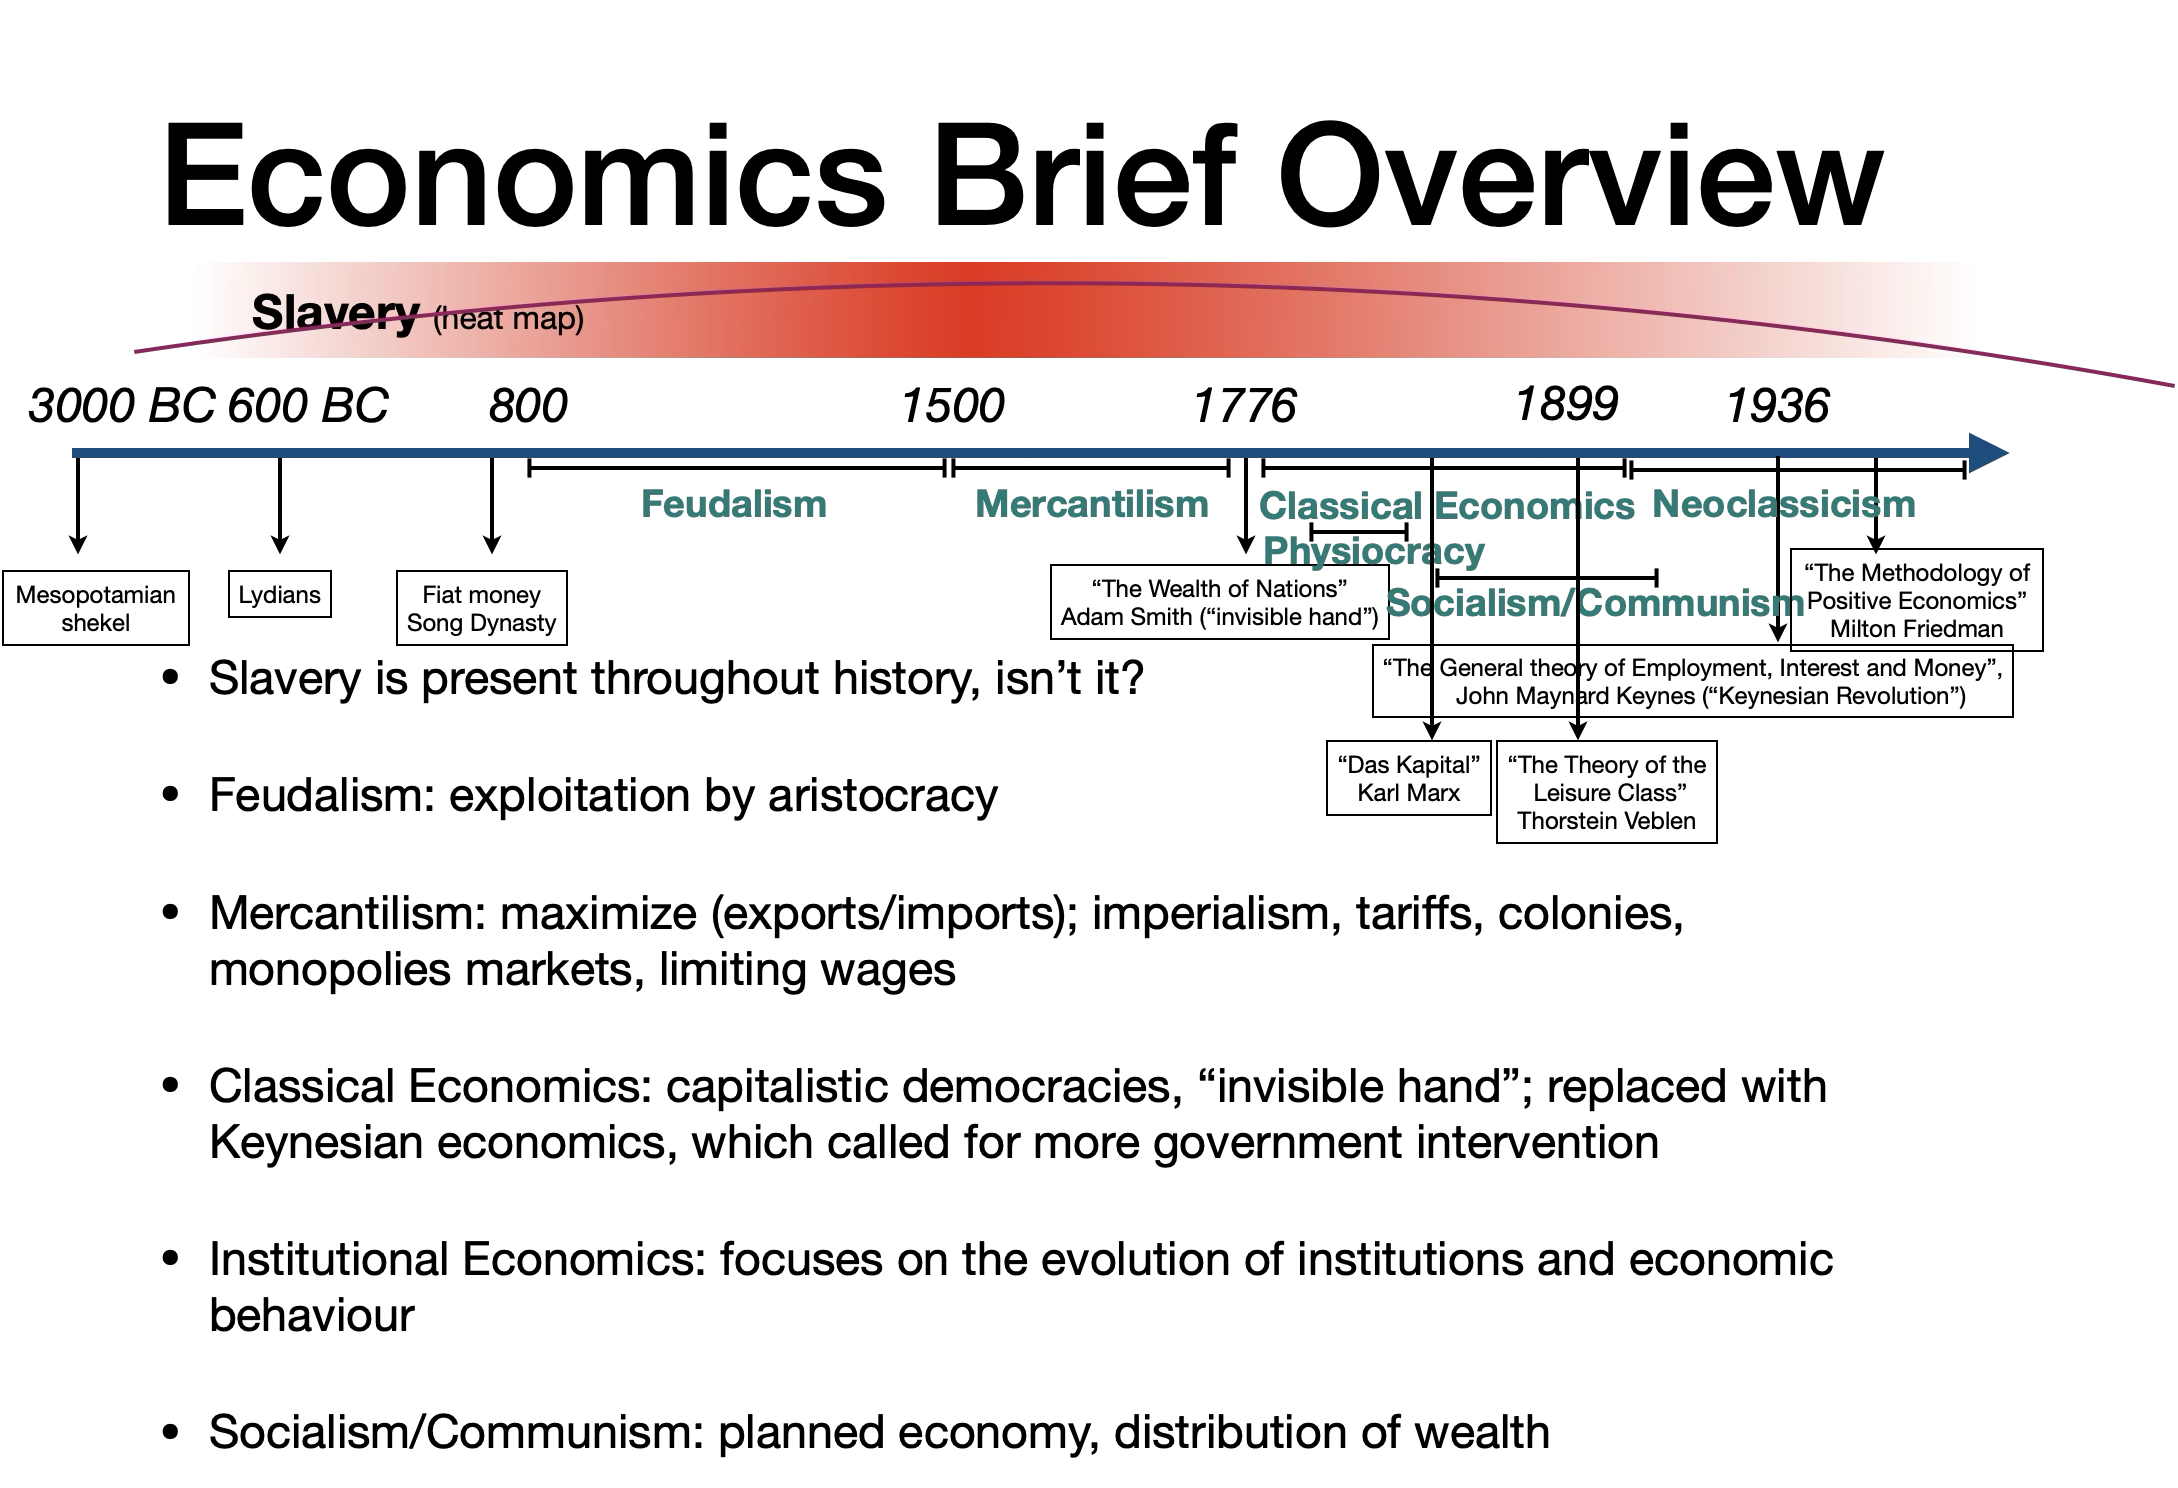
\includegraphics[width=0.9\textwidth]{fig/ses_overview.png}
    \caption{\textbf{Historical Evolution of Socio-Economic Systems}: Brief overview showing transitions from hunter-gatherer societies through agricultural, industrial, and digital economies. Each transition reshaped the consciousness manifold \CC{}.}
    \label{fig:ses_overview}
\end{figure}

\begin{proposition}[SES Evolution and \SYSTEM{} Emergence]
\label{prop:ses_evolution}
\SYSTEM{} is not eternal—it emerged gradually:

\begin{enumerate}
\item \textbf{Pre-agricultural (hunter-gatherer)}: Small bands, egalitarian structures, low \betaDehum{}. \CC{} relatively undistorted (though limited by survival pressures).

\item \textbf{Agricultural Revolution ($\sim$10,000 BCE)}: Surplus enabled hierarchies. Emergence of kings, priests, slaves. \betaDehum{} institutionalized. Birth of \SYSTEM{} in proto-form.

\item \textbf{Industrial Revolution (1800s)}: Capitalism consolidated. Wage labor replaced peasantry. Mass production, urbanization. \SES{} parameters (П1-П5) dramatically shifted toward extraction and control.

\item \textbf{Digital Revolution (1990s-present)}: Platform capitalism, algorithmic control, financialization. \SYSTEM{} achieves unprecedented power due to:
\begin{itemize}
\item Speed (real-time manipulation)
\item Scale (billions connected)
\item Opacity (black-box algorithms)
\end{itemize}
\end{enumerate}

\textbf{Key Inflection: 1970s-1980s}

\begin{itemize}
\item 1971: Dollar-gold decoupling (money supply untethered)
\item 1980s: Neoliberal turn (Reagan, Thatcher) — deregulation, privatization, "trickle-down" ideology
\item Result: Sharp increase in inequality (Fig. \ref{fig:inequality}), financialization, erosion of social safety nets
\end{itemize}

Since then, all five parameters (П1-П5) have trended toward configurations maximizing \SYSTEM{} power and minimizing collective agency.
\end{proposition}

\subsection{Waves and Frequencies: The Temporal Dynamics of \SYSTEM{}}

\begin{figure}[H]
    \centering
    \includegraphics[width=0.85\textwidth]{fig/ses_theory_waves_frequencies.png}
    \caption{\textbf{SES Theory — Waves and Frequencies}: Different \SYSTEM{} dynamics operate at different temporal scales—from millisecond dopamine spikes (neural) to multi-generational trauma patterns (historical). Understanding these frequencies is crucial for designing effective interventions.}
    \label{fig:waves_frequencies}
\end{figure}

\begin{definition}[Temporal Scales of \SYSTEM{} Dynamics]
\label{def:temporal_scales}
\SYSTEM{} operates across multiple timescales:

\begin{itemize}
\item \textbf{Milliseconds-seconds}: Neural firing, dopamine spikes, attention capture
\item \textbf{Minutes-hours}: Social media sessions, work shifts, consumption decisions
\item \textbf{Days-weeks}: Habit formation, news cycles, financial markets
\item \textbf{Months-years}: Career trajectories, election cycles, product lifecycles
\item \textbf{Decades-centuries}: Generational wealth transfer, institutional evolution, cultural paradigms
\item \textbf{Millennia}: Deep historical patterns (e.g., cyclical rise/fall of civilizations)
\end{itemize}

\textbf{Challenge:} Different interventions are required at different scales. Individual therapy addresses neural/behavioral scales; policy reform addresses institutional scales; paradigm shifts address cultural-historical scales.
\end{definition}

% ==========================================
% PART IV: COUNTERACTING SYSTEM
% ==========================================

\section{Part IV: Counteracting \SYSTEM{} Dynamics — The S.V.E. Response}

Understanding \SYSTEM{} is not enough—we must also develop tools to counteract it. This is the purpose of the entire S.V.E. project.

\subsection{Awareness: The Primary Antidote}

\begin{proposition}[Осознанность as Light]
\label{prop:awareness_antidote}
The primary antidote to \SYSTEM{} is \textbf{awareness} (osoznannost' — awareness):

\begin{itemize}
\item Expanding the "lit" regions of \CC{} (Fig. \ref{fig:conscious_unconscious})
\item Reintegrating shadow areas into consciousness
\item Mapping the terrain of \SYSTEM{} so its mechanisms become visible
\end{itemize}

\textbf{Why awareness works:} \SYSTEM{} power depends on unconsciousness (Axiom \ref{ax:unconscious_primacy}). Once patterns are seen, their grip weakens. Like Neo in The Matrix seeing code, or prisoners in the Cave turning to see the fire—awareness is the first step toward liberation.

\textbf{Limitations:} Awareness alone is insufficient if \SES{} parameters remain unchanged (Axiom \ref{ax:ses_embedding}). Thus, awareness must be coupled with action and systemic reform.
\end{proposition}

\subsection{S.V.E. Protocols as Tools for Awareness}

The previous S.V.E. papers (0-XI) introduced specific protocols. We briefly review their role in counteracting \SYSTEM{}:

\subsubsection{S.V.E. X: Cognitive Operating System}

\cite{sve10} The Cognitive OS is a "mental training gym" (trenazher dlya dushi — training gym for the soul), integrating:
\begin{itemize}
\item \textbf{Socrates' Aspect}: Critical thinking, questioning assumptions
\item \textbf{Solomon's Aspect}: Wisdom, long-term thinking, balance
\item \textbf{Ivan's Aspect}: Compassion, empathy, love
\end{itemize}

\textbf{Function in anti-\SYSTEM{} work:}
\begin{itemize}
\item Socrates challenges \SYSTEM{}-generated narratives
\item Solomon resists short-termism (П5)
\item Ivan counteracts \betaDehum{} (reconnects with humanity of "the other")
\end{itemize}

\subsubsection{S.V.E. 0: SIP and Epistemological Boxing}

\cite{sve0} Self-Information-Purification (SIP) and Epistemological Boxing (EBP) provide methods for:
\begin{itemize}
\item Verifying knowledge claims (resisting misinformation)
\item Engaging in rigorous debate (testing theses against counter-arguments)
\item Avoiding dogma (including S.V.E. itself must be tested)
\end{itemize}

\textbf{Relation to \SYSTEM{}:} П3 (Information Control) relies on opacity and narrative management. SIP/EBP counteract by demanding transparency and evidence.

\subsubsection{S.V.E. XI: Verifiable Knowledge Base (VKB)}

\cite{sve11} The VKB is a collaborative system for:
\begin{itemize}
\item Storing verified knowledge with citations
\item Tracking confidence levels and uncertainty
\item Resisting distortion through decentralized verification
\end{itemize}

\textbf{Geometric metaphor:} VKB is a "lighthouse" illuminating dark regions of \CC{}, making \SYSTEM{} dynamics visible.

\subsection{Geodesic Ethics: The Christ-Vector Path}

\cite{sve4, sve8} One of the deepest insights of S.V.E. is the formalization of Jesus Christ's teachings as \textit{geodesic ethics}—the optimal path through the distorted manifold.

\begin{definition}[Christ-Vector]
\label{def:christ_vector}
The \textbf{Christ-Vector} is the geodesic (locally straight path) that:
\begin{enumerate}
\item Maximizes Love (\Love{})
\item Minimizes unnecessary Suffering (\Suffering{})
\item Remains aligned with Truth (does not compromise integrity for comfort)
\end{enumerate}

On an undistorted manifold, this would be a straight line. On the Fall-distorted \CC{}, it requires navigating curvature—"taking up one's cross."
\end{definition}

\begin{proposition}[Jesus as Cartographer of the Fall]
\label{prop:jesus_cartographer}
Jesus's teachings (forgiveness, love of enemies, "turn the other cheek," "the truth shall set you free") can be understood as \textit{instructions for navigating the Fall-distorted manifold}:

\begin{itemize}
\item \textbf{Forgiveness}: Breaks cycles of retaliation (prevents \betaDehum{} feedback loops)
\item \textbf{Love of enemies}: Resists tribal in-group/out-group dynamics (heals fragmentation)
\item \textbf{Turn the other cheek}: Absorbs violence without perpetuating it (damping oscillations)
\item \textbf{Truth as liberation}: Awareness dispels illusions (escaping the Cave)
\item \textbf{"I am the Way, the Truth, and the Life"}: Christ-Vector as the geodesic path
\end{itemize}

\textbf{Key insight:} This is not about theology or supernatural claims but about \textit{psychological and geometric truth}. The teachings work because they align with the actual structure of \CC{} and counteract Fall distortions.
\end{proposition}

\begin{remark}[Non-Sectarian Interpretation]
S.V.E. respects all wisdom traditions. The Christ-Vector is named after Jesus because his teachings provide exceptionally clear articulation of geodesic ethics. However, similar principles appear in Buddhism (compassion, non-attachment), Stoicism (virtue, equanimity), and other traditions. The goal is \textit{integration of wisdom}, not conversion to Christianity.
\end{remark}

\subsection{Reforming SES: Towards "Capitalism 2.0"}

Awareness and individual practice are necessary but insufficient. We must also reform \SES{} parameters (П1-П5).

\subsubsection{The PEMY Model}

PEMY (\textbf{P}arent-\textbf{E}lder-\textbf{M}iddle-\textbf{Y}oung) is a proposed business model that aims to realign incentives and reshape the consciousness manifold.

\begin{definition}[PEMY Business Model]
\label{def:pemy}
PEMY reimagines corporate structure and ownership:

\textbf{Traditional Model (current \SES{}):}
\begin{itemize}
\item Founders/VCs own majority shares
\item Profit maximization is sole objective
\item Workers are "human resources" (disposable)
\item Community/environment are externalities (ignored)
\end{itemize}

\textbf{PEMY Model:}
\begin{itemize}
\item \textbf{Parent (Top 1\% / Founding Visionaries)}: 20-30\% ownership. Responsible for long-term vision, strategic decisions, but do not dominate.
\item \textbf{Elder Children (Senior Contributors)}: 20-25\% ownership. Experienced team members, mentors.
\item \textbf{Middle Children (Main Workforce)}: 25-30\% ownership. All employees are shareholders—aligned incentives.
\item \textbf{Young Children (Community / Customers)}: 20-30\% ownership. Those served by the company have a stake in its governance.
\end{itemize}

\textbf{Key Features:}
\begin{enumerate}
\item \textbf{Shared Ownership}: Everyone is a stakeholder, not just capital providers.
\item \textbf{Transparency}: Monthly financial reports, annual assemblies, open governance.
\item \textbf{Multi-Objective Optimization}: Goals include not just profit but:
\begin{itemize}
\item Employee well-being and work-life balance
\item Environmental sustainability
\item Community benefit
\item Knowledge/skill development
\end{itemize}
\item \textbf{Long-Term Orientation}: Quarterly earnings pressure is eliminated; focus shifts to sustainable value creation.
\end{enumerate}
\end{definition}

\begin{figure}[H]
    \centering
    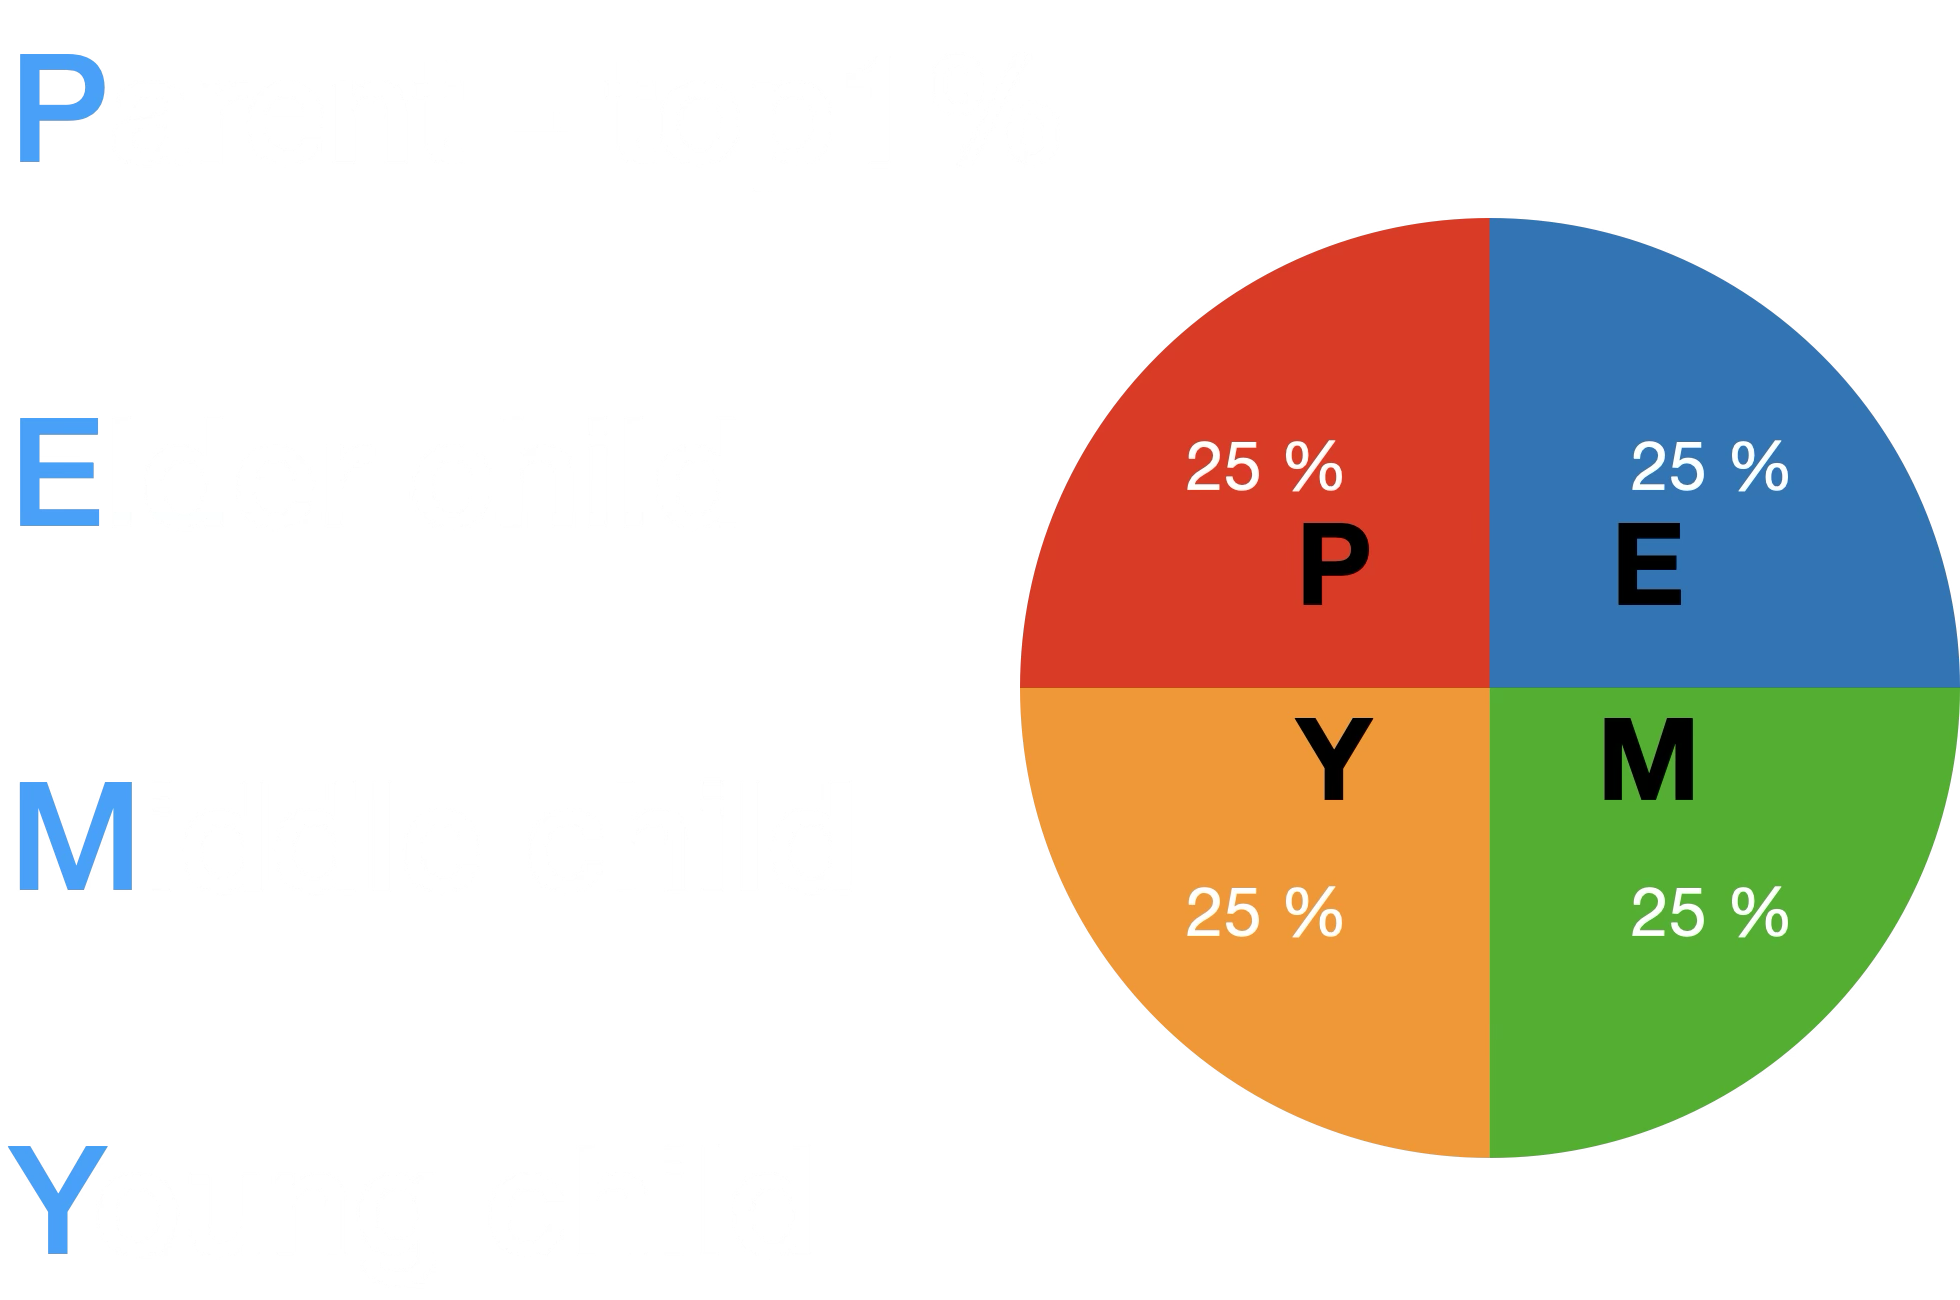
\includegraphics[width=0.8\textwidth]{fig/pemy_part_1.png}
    \caption{\textbf{PEMY Business Model — Part 1}: Overview of the Parent-Elder-Middle-Young ownership structure, contrasting with traditional capitalist models.}
    \label{fig:pemy1}
\end{figure}

\begin{figure}[H]
    \centering
    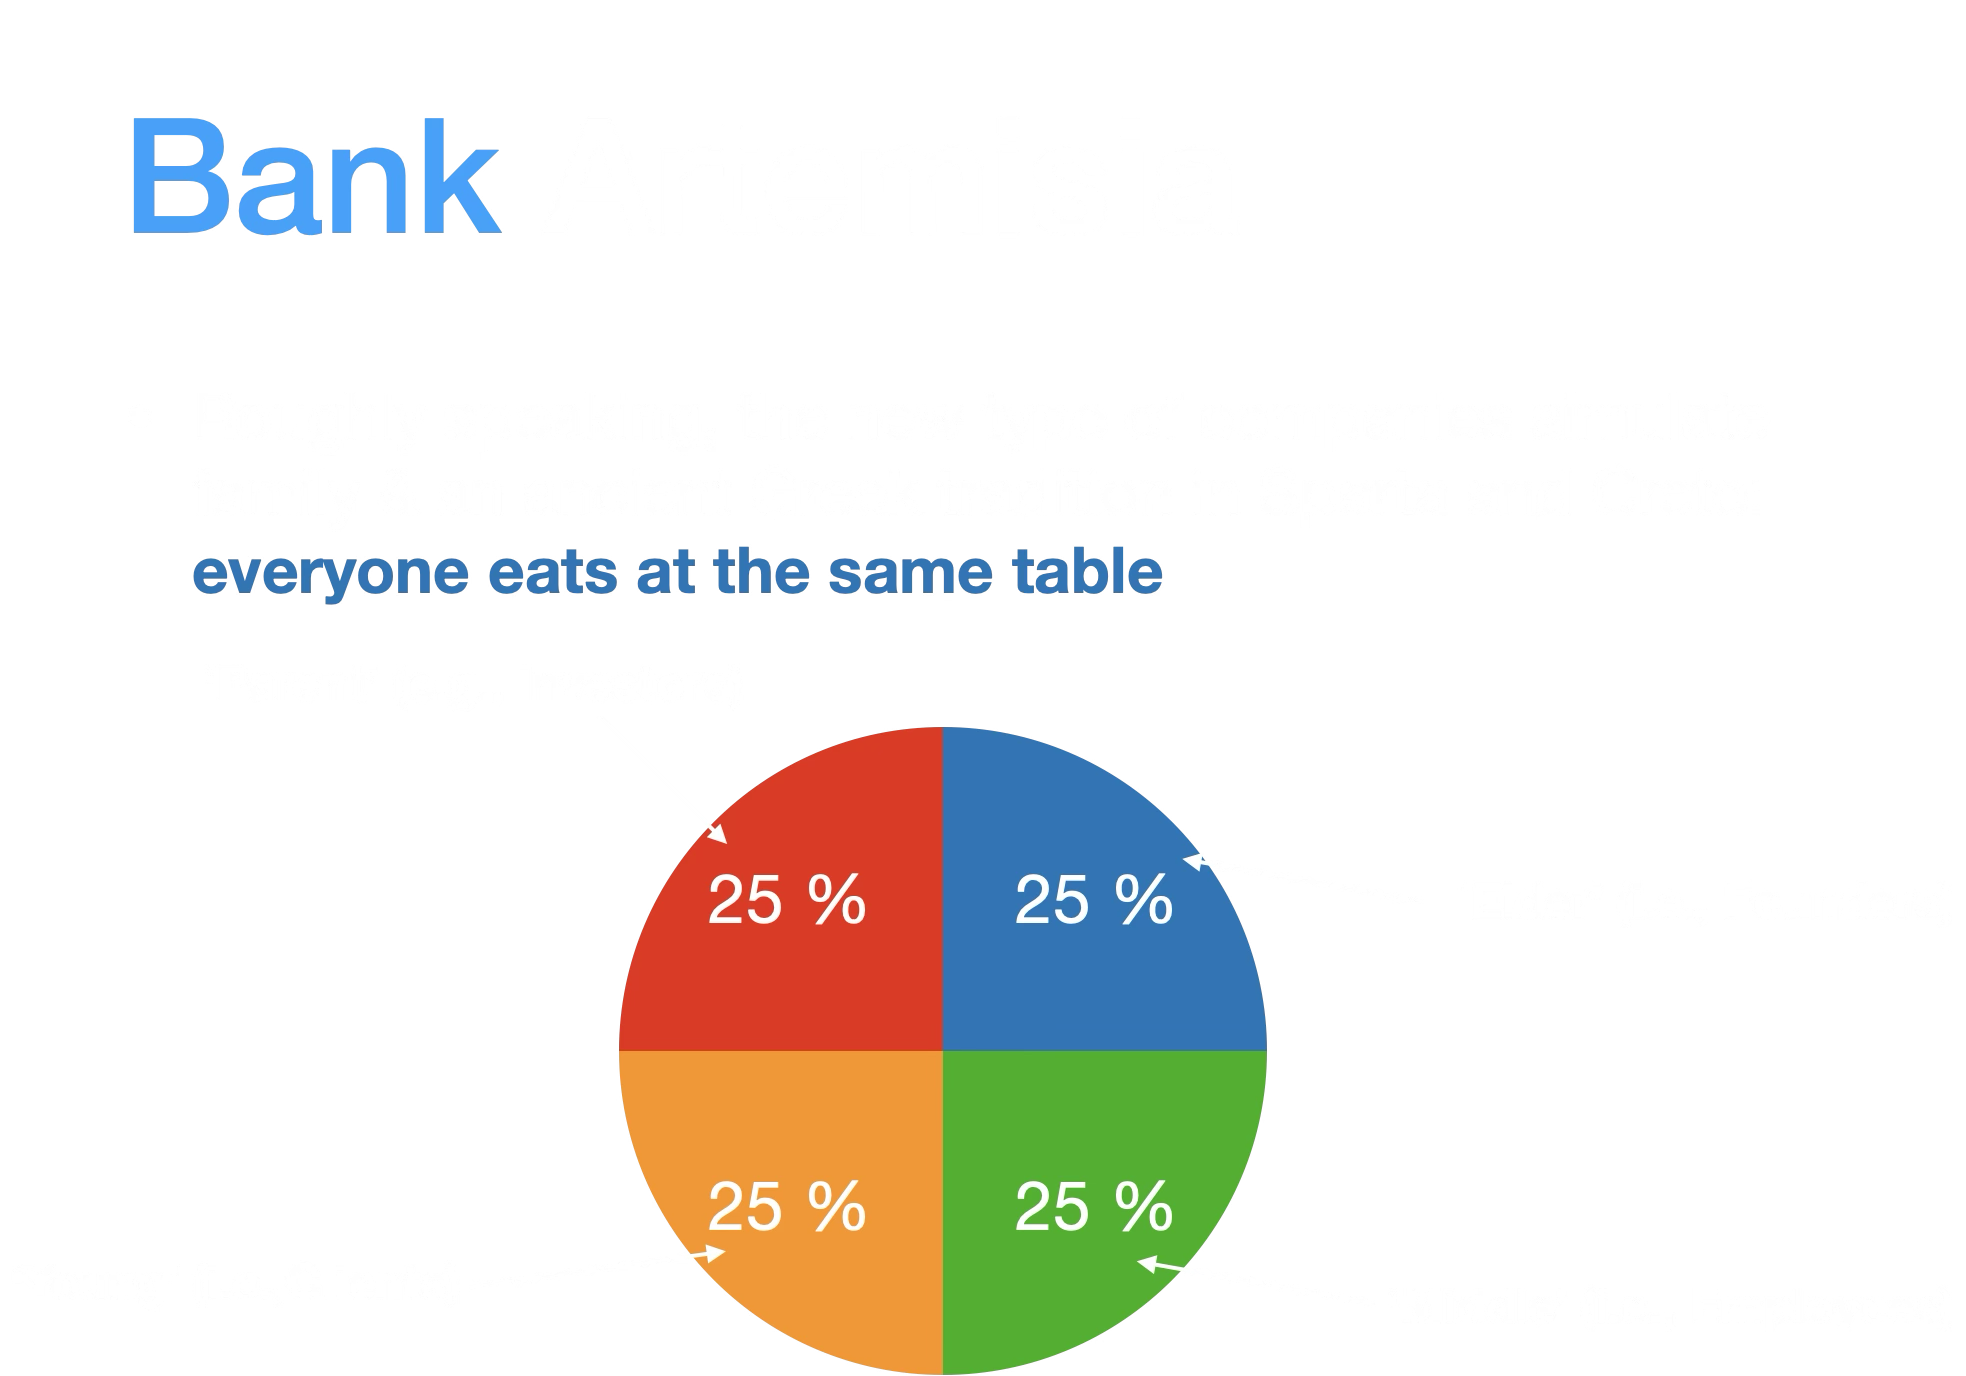
\includegraphics[width=0.8\textwidth]{fig/pemy_part_2.png}
    \caption{\textbf{PEMY Business Model — Part 2 (Bank Artemisia Example)}: Concrete example of how PEMY principles apply to a bank. Every client is a shareholder; the bank's goal is to improve quality of life for all shareholders, not just extract maximum profit.}
    \label{fig:pemy2}
\end{figure}

\begin{example}[Bank Artemisia — PEMY in Practice]
Imagine a bank structured under PEMY principles:
\begin{itemize}
\item \textbf{Ownership}: Every account holder is a micro-shareholder.
\item \textbf{Governance}: Annual general assembly where representatives discuss key decisions.
\item \textbf{Transparency}: Monthly financial reports sent to all shareholders.
\item \textbf{Goals}: Not just profit, but:
\begin{enumerate}
\item Provide fair, transparent financial services
\item Support local economy (loans to small businesses, sustainable projects)
\item Educate shareholders about finance
\item Maintain work-life balance for employees
\end{enumerate}
\item \textbf{Anti-Abuse}: With such transparency, misusing client data becomes impossible (shareholders would revolt).
\end{itemize}

\textbf{Comparison to Current Banks:}
\begin{itemize}
\item \textbf{Current}: Shareholders are distant investors (often institutional funds); clients are revenue sources; workers are cost centers.
\item \textbf{PEMY}: Shareholders = clients = workers (overlapping circles). Aligned incentives across all stakeholders.
\end{itemize}
\end{example}

\begin{figure}[H]
    \centering
    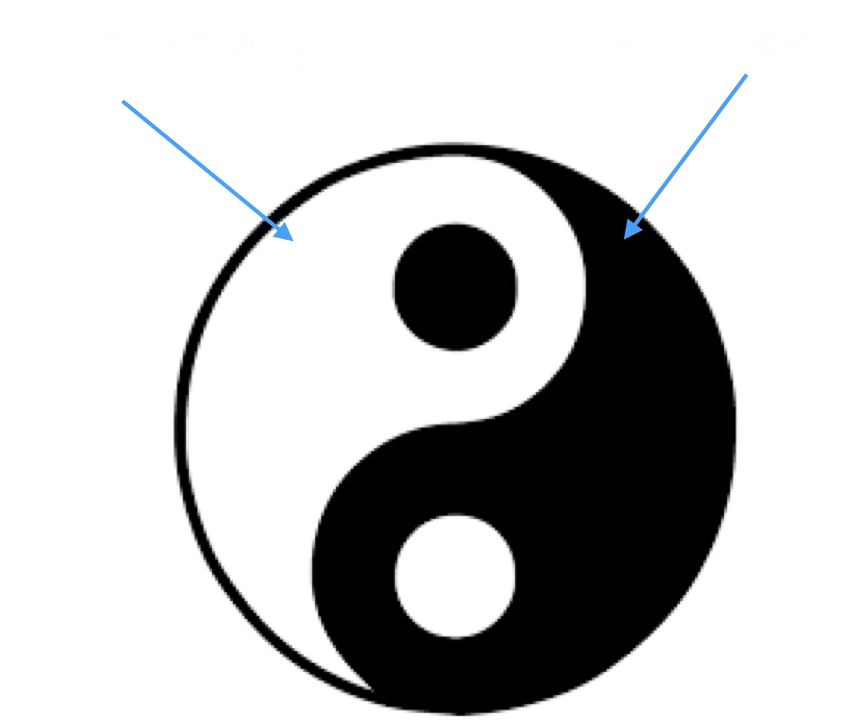
\includegraphics[width=0.85\textwidth]{fig/inyan_uber_type1_type2_PEMY.png}
    \caption{\textbf{Yin-Yang: Traditional Uber vs. PEMY Uber}: Illustration of two Uber models coexisting—traditional (profit-maximizing, extractive) and PEMY (cooperative, stakeholder-aligned). They are complementary, not mutually exclusive. The PEMY model offers an alternative for those who value ethics and sustainability.}
    \label{fig:pemy_uber}
\end{figure}

\begin{figure}[H]
    \centering
    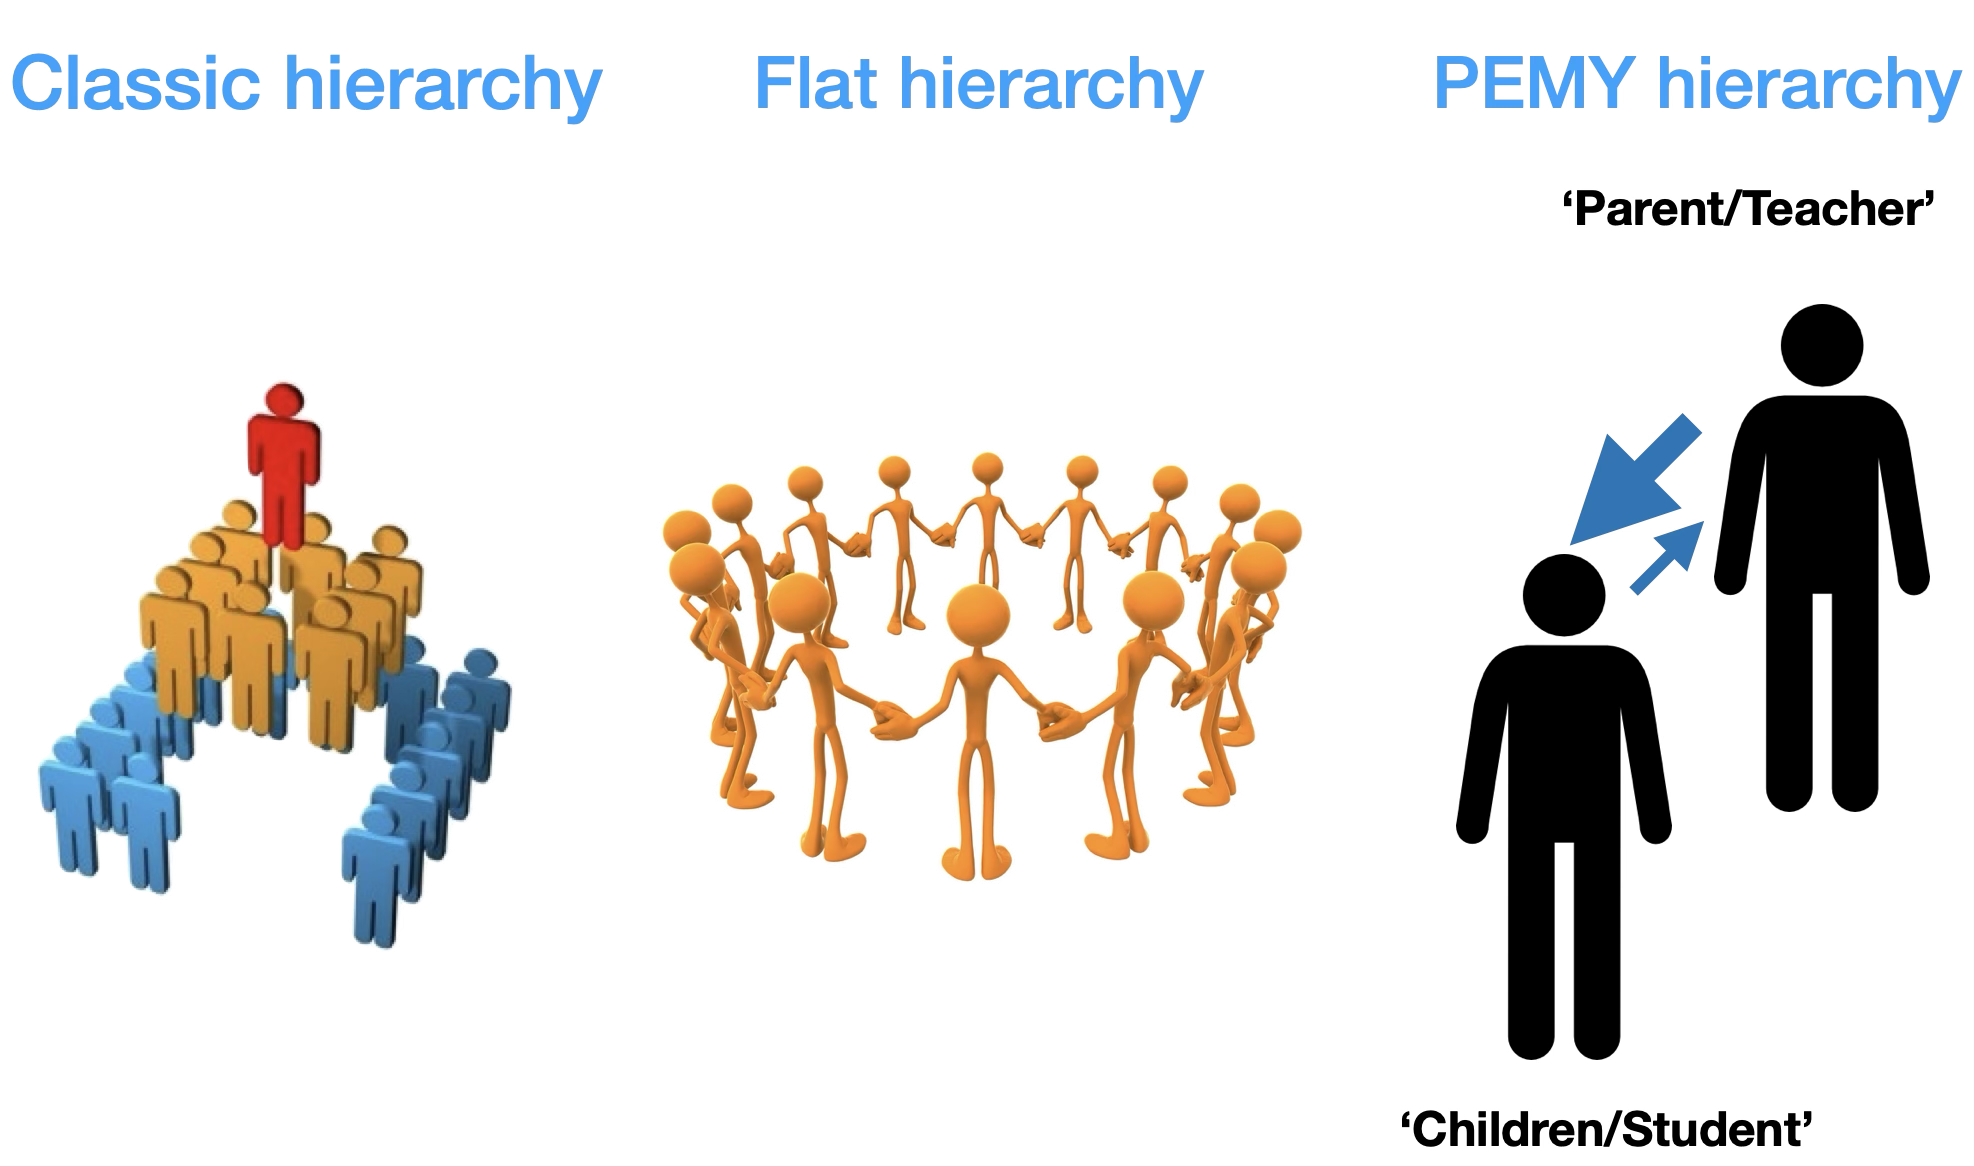
\includegraphics[width=0.7\textwidth]{fig/pemy_part_3_hierarchy.png}
    \caption{\textbf{PEMY Hierarchy vs. Alternatives}: Comparison of PEMY (family-like, balanced hierarchy) with flat structures (leaderless chaos) and pyramidal structures (authoritarian, top-heavy). PEMY aims for optimal balance between autonomy and coordination.}
    \label{fig:pemy_hierarchy}
\end{figure}

\subsubsection{How PEMY Reshapes \SES{} Parameters}

\begin{proposition}[PEMY Impact on П1-П5]
\label{prop:pemy_impact}
If widely adopted, PEMY would transform all five parameters:

\begin{itemize}
\item \textbf{П1 (Incentive Alignment)}: Shared ownership aligns individual and collective interests. Workers care about long-term health because they benefit directly.

\item \textbf{П2 (Resource Distribution)}: Profits distributed among all stakeholders, reducing concentration. Wealth grows more evenly.

\item \textbf{П3 (Information Control)}: Transparency requirement breaks information asymmetry. Algorithmic decisions would be explainable; governance would be participatory.

\item \textbf{П4 (Transparency \& Accountability)}: Built-in by design. Open reports, assemblies, verifiable records.

\item \textbf{П5 (Temporal Orientation)}: Elimination of quarterly pressure allows long-term focus. Sustainable practices become profitable.
\end{itemize}

\textbf{Geometric Consequence:} PEMY reshapes the curvature of \CC{}. Paths toward cooperation, transparency, and long-term thinking become "downhill" (low resistance), while paths toward exploitation become "uphill" (high cost).
\end{proposition}

\begin{remark}[Transition Challenges]
Implementing PEMY faces enormous resistance:
\begin{itemize}
\item Current elites benefit from status quo (П2 concentration)
\item Legal frameworks favor traditional corporate structures
\item Cultural inertia ("greed is good," "there is no alternative")
\item Coordination problem (first movers may be outcompeted by ruthless incumbents)
\end{itemize}

\textbf{Strategies for Transition:}
\begin{enumerate}
\item Start with pilot projects (e.g., cooperative tech startups, community banks)
\item Build evidence of viability (demonstrate that PEMY can compete)
\item Create legal infrastructure (B-corps, social enterprises as stepping stones)
\item Cultural shift (via education, media, S.V.E. dissemination)
\item Critical mass (once enough entities adopt, network effects favor PEMY)
\end{enumerate}
\end{remark}

\subsection{Awakening Empathy in Elites: Breaking the Hostage Dynamic}

As discussed, elites are also "hostages" of \SYSTEM{}. A crucial question: How can we awaken their awareness?

\begin{proposition}[Elites as System Hostages]
\label{prop:elites_hostage}
Most individuals in the "1\%" or "0.01\%" are \textit{not consciously malicious}. They are products of:
\begin{itemize}
\item Privileged upbringing (normalized wealth inequality)
\item Elite education (emphasizing status competition, "meritocracy" myths)
\item Professional environments (incentivizing ruthlessness)
\item Psychological defenses (rationalization, moral disengagement)
\end{itemize}

\textbf{Thought Experiment:} If an "average" person were raised in the same circumstances (elite schools, inherited wealth, constant reinforcement of superiority), would they behave differently? Most likely not. This is not to excuse harm but to recognize its \textit{systemic} nature (Axiom \ref{ax:ses_embedding}).

\textbf{Implication:} Vilifying individuals misses the point. We must (1) hold them accountable for actions, but (2) offer paths to redemption and transformation.
\end{proposition}

\begin{proposition}[Direct Experience as Transformative Tool]
\label{prop:direct_experience}
One of the most powerful ways to break \betaDehum{} and awaken empathy is \textit{direct, embodied experience} of suffering caused by one's actions or system.

\textbf{Proposal:} Mandate (or strongly encourage) that individuals in elite positions—politicians, CEOs, military commanders—spend time (e.g., final year of elite schooling, or sabbatical) in regions/communities directly affected by "Satanic Chess" decisions.

\textbf{Examples:}
\begin{itemize}
\item Young investment bankers spending months in communities devastated by predatory lending
\item Defense contractors' children volunteering in war-torn regions
\item Tech executives living without digital access for extended periods
\item Political leaders living on minimum wage in their own countries
\end{itemize}

\textbf{Mechanism:} Direct contact with "the other" as full humans (not abstractions, metrics, or enemies) pierces \betaDehum{}. Empathy is difficult to sustain across distance and abstraction but emerges naturally through proximity and shared experience.

\textbf{Personal Testimony:} The author (Artiom Kovnatsky) experienced the collapse of the USSR, hunger, violence, emigration, and the "love and attention of the White Man" (irony intended). These experiences cannot be conveyed through text alone—they must be \textit{felt}. This is why direct experience is so powerful and why \SYSTEM{} works so hard to prevent it (segregation, gated communities, media bubbles).
\end{proposition}

\begin{remark}[Practical Challenges]
Implementing such programs faces obstacles:
\begin{itemize}
\item \SYSTEM{} will resist (threatens its perpetuation)
\item Concerns about "safety" (real and manufactured)
\item Risk of tokenism (performative visits without genuine engagement)
\item Psychological resistance (elites' ego defenses)
\end{itemize}

\textbf{Yet:} Even partial implementation could have transformative effects. A single CEO or politician genuinely awakened could shift entire organizations or policies.
\end{remark}

\begin{remark}[Additional Insights]
Beyond direct experience, consider:

\begin{enumerate}
\item \textbf{"Stockholm Syndrome" of Elites:} Some elites develop psychological dependency on \SYSTEM{} (it gives them identity, power, meaning). They may \textit{defend} it even when intellectually recognizing its harm. Addressing this requires therapeutic approaches (integrating shadow, grieving loss of false self).

\item \textbf{Role of Redemption:} S.V.E. must offer elites not just critique but a \textit{positive role} in transformation. E.g., using wealth to fund VKB, PEMY startups, or education reform. "If not us, then who?" applies to them too.

\item \textbf{"Translation" of S.V.E.:} Ideas must be framed in language elites understand—risk management, long-term stability, legacy, even self-interest (extreme inequality threatens social cohesion, which threatens their security). S.V.E. should not compromise truth but can adapt presentation.
\end{enumerate}
\end{remark}

\subsection{Summary of Anti-\SYSTEM{} Strategies}

\begin{table}[H]
\centering
\caption{Multi-Level Interventions Against \SYSTEM{}}
\label{tab:interventions}
\begin{tabular}{@{}lll@{}}
\toprule
\textbf{Scale} & \textbf{Tool/Strategy} & \textbf{S.V.E. Reference} \\ \midrule
Neural/Psychological & Cognitive OS training & S.V.E. X \cite{sve10} \\
 & Meditation, shadow work & Jung, S.V.E. XII \\
Interpersonal & Empathy practices & Ivan aspect, S.V.E. X \\
 & Direct experience programs & S.V.E. XII \S 4.5 \\
Informational & VKB, SIP, EBP & S.V.E. XI, 0 \cite{sve11, sve0} \\
Organizational & PEMY business models & S.V.E. XII \S 4.4 \\
 & Cooperative structures & \\
Policy/Legal & Regulation of platforms & \\
 & Wealth redistribution & \\
 & Campaign finance reform & \\
Cultural/Paradigm & Education reform & S.V.E. XII \S 2.3 \\
 & Media literacy & \\
 & S.V.E. dissemination & All S.V.E. works \\
Ethical/Spiritual & Christ-Vector alignment & S.V.E. IV, VIII \cite{sve4, sve8} \\
 & Geodesic ethics & S.V.E. XII \S 4.3 \\ \bottomrule
\end{tabular}
\end{table}

% ==========================================
% PART V: CONCLUSION & CHALLENGE
% ==========================================

\section{Conclusion: Towards Collective Self-Awareness and the Call to Action}

\subsection{Summary of the \SYSTEM{} Model}

We have presented \SYSTEM{} as a comprehensive, geometrically formalized model of collective unconscious dynamics. Key components:

\begin{enumerate}
\item \textbf{Theoretical Foundation}:
\begin{itemize}
\item Integration of Jung's collective unconscious, Smith's invisible hand, Plato's Cave
\item Consciousness manifold \CC{} as geometric space
\item The Fall as curvature distortion
\item \betaDehum{} as systemic dehumanization
\end{itemize}

\item \textbf{Three Foundational Axioms}:
\begin{itemize}
\item A1: Unconscious Primacy (most behavior is unconscious)
\item A2: Socio-Economic Embedding (unconscious shaped by \SES{})
\item A3: Emergent Autonomy (\SYSTEM{} self-perpetuates)
\end{itemize}

\item \textbf{Five SES Parameters (П1-П5)}:
\begin{itemize}
\item П1: Incentive Alignment
\item П2: Resource Distribution
\item П3: Information Asymmetry
\item П4: Transparency \& Accountability
\item П5: Temporal Orientation
\end{itemize}

\item \textbf{Concrete Manifestations}:
\begin{itemize}
\item Dollar/gold decoupling, wealth concentration, digitization
\item Education, social media, "Satanic Chess," trauma-driven policies
\item Historical examples (SPE, Tuskegee, Iraq War)
\end{itemize}

\item \textbf{Counterstrategies}:
\begin{itemize}
\item Awareness (osoznannost' — awareness) as light
\item S.V.E. protocols (Cognitive OS, VKB, SIP/EBP)
\item Christ-Vector geodesic ethics
\item PEMY business models (Capitalism 2.0)
\item Empathy awakening (including elites)
\end{itemize}
\end{enumerate}

\begin{figure}[H]
    \centering
    \includegraphics[width=0.7\textwidth]{fig/where_humanity_goes.png}
    \caption{\textbf{Where is Humanity Going?} (Illustration from Russian animation "Hedgehog in the Fog"): A lone figure moving through obscurity toward an uncertain destination. This captures the current human condition—stumbling through \SYSTEM{}-generated fog. S.V.E. offers a map and compass.}
    \label{fig:where_humanity_goes}
\end{figure}

\subsection{The Einstein Imperative: Rational Knowledge Over Fear and Faith}

\begin{mdframed}[backgroundcolor=gray!10]
\textbf{The Einstein Imperative:}

\begin{center}

\textit{"The further the spiritual evolution of mankind advances, the more certain it seems to me that the path to genuine religiosity does not lie through the fear of life, and the fear of death, and blind faith, but through striving after rational knowledge."}

--- \textbf{Albert Einstein} \cite{einstquote}
\end{center}

S.V.E., with its focus on rational knowledge, logic, verification, and mathematical rigor, offers precisely this path advocated by Einstein—a way towards genuine understanding free from the fear and blind faith often exploited by \SYSTEM{}.
\end{mdframed}

\begin{figure}[H]
    \centering
    \includegraphics[width=0.55\textwidth]{fig/einstein_quote.png}
    \caption{\textbf{Einstein Quote (Visual)}: The full quote emphasizing rational knowledge over fear-based belief systems. This is the philosophical north star of S.V.E.}
    \label{fig:einstein_quote}
\end{figure}

\subsection{The Challenge to Academia and Humanity}

We now issue a formal challenge:

\begin{mdframed}[linecolor=svered, linewidth=2pt, backgroundcolor=gray!5]
\textbf{Challenge to the Global Academic and Intellectual Community:}

\begin{enumerate}
\item \textbf{Refute S.V.E.:} Demonstrate internal contradictions or factual inaccuracies in the \SYSTEM{} model using its own standards of rigor (mathematical formalization per S.V.E. VIII \cite{sve8}, verification protocols per S.V.E. IX \cite{sve9}).

\item \textbf{Improve upon S.V.E.:} Propose an alternative model that:
\begin{itemize}
\item Explains the same range of phenomena (from individual psychology to global economics)
\item Provides equal or greater explanatory power
\item Offers comparable or superior mathematical/logical formalization
\item Includes protocols for verification and falsification
\end{itemize}

\item \textbf{Engage via Epistemological Boxing (EBP):} Any critic claiming S.V.E. is "pseudoscience," "theology," "unfalsifiable," or "unfounded" is invited to a public EBP match \cite{sve0}. Let us test both theses under S.V.E.'s own rules of engagement:
\begin{itemize}
\item Clearly defined propositions
\item Explicit evidence standards
\item Logical argumentation
\item Good faith dialectic (seeking truth, not victory)
\end{itemize}
May new knowledge arise from this contest.

\item \textbf{Use S.V.E.:} If no superior alternative is presented and S.V.E. withstands critique, then begin \textit{using} S.V.E. tools (Cognitive OS \cite{sve10}, VKB \cite{sve11}, SIP/EBP \cite{sve0}, PEMY models) to diagnose and address real-world problems driven by \SYSTEM{}.
\end{enumerate}
\end{mdframed}

\subsection{Does an Alternative Exist?}

To our knowledge, no widely accepted framework integrates:
\begin{itemize}
\item Individual psychology (Jung, Freud, neuroscience)
\item Economic dynamics (Smith, Marx, behavioral economics)
\item Systemic analysis (complexity theory, emergence)
\item Ethical guidance (Christ-Vector, geodesic ethics)
\item Practical tools (VKB, PEMY, Cognitive OS)
\end{itemize}
into a \textit{unified, mathematically formalized, falsifiable} model.

Existing theories explain \textit{parts}:
\begin{itemize}
\item Economics explains resource allocation (but ignores psychological unconscious)
\item Psychology explains individual behavior (but ignores systemic constraints)
\item Marxism explains class struggle (but lacks geometric formalization and individualist tools)
\item Religion offers ethical guidance (but often rejects rational inquiry)
\end{itemize}

\textbf{S.V.E. attempts synthesis.}

\textbf{If you know of a better model, please share it.} We are not dogmatic—S.V.E. is version 0.x, a work in progress. However, dismissing S.V.E. as "speculative" without offering a superior alternative is intellectually insufficient.

Any model is an approximation; its value lies in \textit{utility}. If S.V.E. currently offers the most coherent, potentially verifiable, integrated picture, then it deserves serious consideration.

\subsection{Return to Philosophical Roots: If Not Us, Then Who?}

Let us recall our lineage:

\begin{itemize}
\item \textbf{Socrates} fought for Athens in battle, not just in the marketplace. He valued physical courage alongside intellectual rigor. He drank hemlock rather than compromise truth.
\item \textbf{Plato} was a wrestler and soldier before becoming a philosopher. He understood that philosophy must be \textit{lived}, not just theorized.
\end{itemize}

They sought \textbf{Truth in Life}, not just in abstract academia.

\textbf{A Question for Modern Academia:} Have we retreated behind institutional walls, generating \SYSTEM{}-serving noise (publish-or-perish, grant-chasing, jargon-laden irrelevance) instead of being a \textbf{"Lighthouse for Humanity"} (Mayak dlya Chelovechestva — Lighthouse for Humanity)?

Perhaps it is time to:
\begin{enumerate}
\item Confront our own place within \SYSTEM{} (how universities are captured, how research is commodified)
\item Reclaim the \textit{active, courageous} pursuit of Truth
\item Engage with the world's suffering, not as detached observers but as participants in its healing
\end{enumerate}

\textbf{Esli ne my, to kto? — If not us, then who?} \\
\textbf{If not us, then who?}

\subsection{S.V.E. as Hypothesis v0.x — Invitation to Co-Creation}

The S.V.E. framework, including the \SYSTEM{} model, is presented \textit{not as dogma} but as:
\begin{itemize}
\item A \textbf{hypothesis} (version 0.x) inviting rigorous testing
\item A \textbf{work in progress}, open to refinement
\item An \textbf{invitation to collaboration}—join us in improving it
\end{itemize}

The author (Dr. Artiom Kovnatsky) commits to:
\begin{itemize}
\item Using constructive critique to refine S.V.E. toward version 0.9 (and eventually 1.0)
\item Operating in good faith, with humility about our limitations
\item Serving Truth "dlya pol'zy Chelovekov — for the benefit of Humans" (for the benefit of Humans)
\end{itemize}

\textbf{This is not my work alone—it is ours.} S.V.E. synthesizes millennia of human wisdom (Plato, Jesus, Jung, Einstein, Russell, and countless others). It is humanity's collective project to understand itself and transcend its limitations.

\subsection{Final Reflections and Blessings}

We live in a time of unprecedented danger and unprecedented opportunity:
\begin{itemize}
\item \textbf{Danger}: Ecological collapse, nuclear weapons, AI alignment, social fragmentation, mental health crises—all symptoms of \SYSTEM{} dynamics run amok.
\item \textbf{Opportunity}: Global connectivity, accumulated knowledge, technological tools, and growing awareness create possibilities for transformation never before available.
\end{itemize}

The path forward requires:
\begin{enumerate}
\item \textbf{Awareness} (osoznannost' — awareness): Illuminating shadow regions of \CC{}
\item \textbf{Courage}: Confronting uncomfortable truths about ourselves and our systems
\item \textbf{Love}: Extending empathy even to "enemies" (recognizing them as fellow hostages)
\item \textbf{Action}: Reforming \SES{} structures (PEMY, VKB, policy changes)
\item \textbf{Integration}: Bringing conscious and unconscious into dialogue (Jung's individuation at collective scale)
\end{enumerate}

This is the S.V.E. path—from fragmentation toward wholeness, from fear toward love, from \SYSTEM{}-driven chaos toward conscious co-creation.

\vspace{1em}

\begin{center}

\textbf{S Bogom! — With God!} (For those who believe) \\

\textbf{With Love} (For all)!
\end{center}

\vspace{1em}

\textit{May this work serve Truth and contribute to the healing of our shared consciousness.}

% --- BIBLIOGRAPHY ---
\newpage
\bibliographystyle{plainnat}
\bibliography{\jobname}

% --- APPENDICES ---
\newpage
\appendix

\section{Summary of \SYSTEM{} Axioms}

\begin{table}[H]
\centering
\caption{The Three Foundational Axioms of \SYSTEM{}}
\begin{tabular}{@{}p{0.2\textwidth}p{0.7\textwidth}@{}}
\toprule
\textbf{Axiom} & \textbf{Description} \\ \midrule
\textbf{A1: Unconscious Primacy} & The majority of human behavior is driven by unconscious processes (biases, fears, desires) operating below awareness. Conscious thought is often post-hoc rationalization. \\[0.3cm]
\textbf{A2: Socio-Economic Embedding} & Unconscious patterns are shaped, reinforced, and transmitted through socio-economic structures (\SES{}). To change consciousness, we must change \SES{} parameters (П1-П5). \\[0.3cm]
\textbf{A3: Emergent Autonomy} & Once established, \SYSTEM{} exhibits quasi-autonomous dynamics, perpetuating itself through feedback loops, institutional capture, and resistance to disruption. \\ \bottomrule
\end{tabular}
\end{table}

\section{Summary of \SES{} Parameters}

\begin{table}[H]
\centering
\caption{The Five Key Parameters of Socio-Economic Systems}
\begin{tabular}{@{}p{0.25\textwidth}p{0.65\textwidth}@{}}
\toprule
\textbf{Parameter} & \textbf{Description} \\ \midrule
\textbf{П1: Incentive Alignment} & Degree to which rewards align individual behavior with collective well-being. Current systems are highly misaligned (rewarding extraction). PEMY aims for alignment. \\[0.3cm]
\textbf{П2: Resource Distribution} & Concentration vs. dispersion of wealth/power. Measured by Gini coefficient, wealth ratios. Currently: extreme concentration (top 1\% holds 35\%+ of wealth). \\[0.3cm]
\textbf{П3: Information Asymmetry \& Control} & Privileged access to information/narratives. Manifests as media concentration, algorithmic curation, educational gatekeeping. Creates artificial curvature in \CC{}. \\[0.3cm]
\textbf{П4: Transparency \& Accountability} & Visibility of power structures and enforcement of ethics. Low transparency = high \SYSTEM{} freedom. PEMY mandates transparency by design. \\[0.3cm]
\textbf{П5: Temporal Orientation} & Time horizon privileged by incentives (short vs. long term). Current bias: extreme short-termism (quarterly earnings, dopamine hits). Consequences: ecological/social collapse. \\ \bottomrule
\end{tabular}
\end{table}

\section{Additional Illustrative Figures}

% Include any remaining figures mentioned in the file lists that weren't already placed in the main text

\begin{figure}[H]
    \centering
    \includegraphics[width=0.85\textwidth]{fig/S_V_E_universe_1_9.pdf}
    \caption{\textbf{S.V.E. Universe Overview (Papers 0-9)}: Brief summary of the S.V.E. series prior to Papers X, XI, and XII. Shows the progression from foundational epistemology (S.V.E. 0) through mathematical formalization (S.V.E. VIII) to verification protocols (S.V.E. IX).}
    \label{fig:sve_overview}
\end{figure}

\begin{figure}[H]
    \centering
    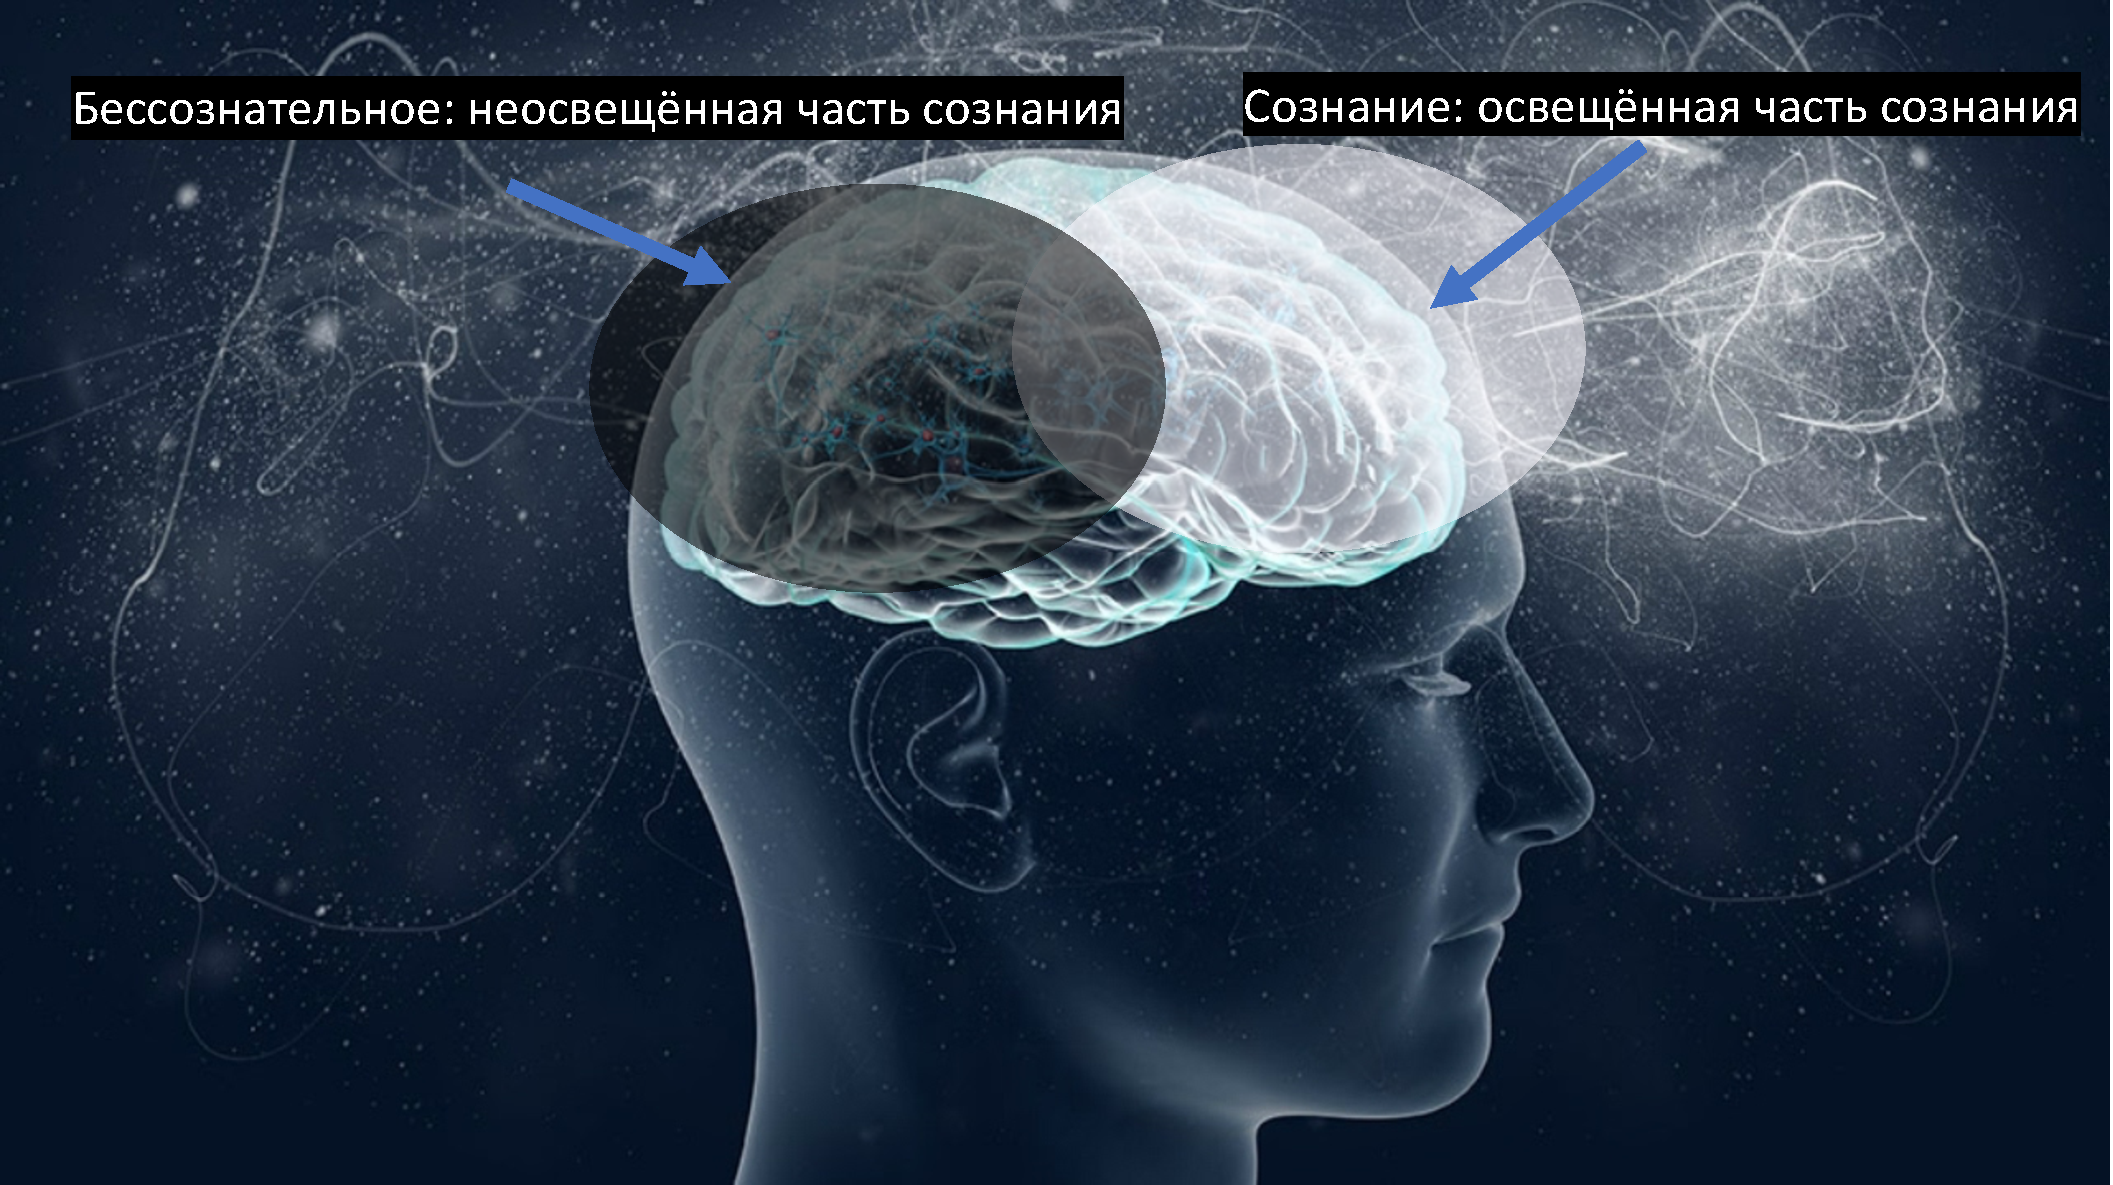
\includegraphics[width=0.7\textwidth]{fig/model_conciousness_subconsiousness.pdf}
    \caption{\textbf{Model of Consciousness and Subconsciousness}: Another representation of the light/shadow dynamics in the human psyche, showing how attention (light) illuminates only portions of the vast unconscious terrain.}
    \label{fig:consciousness_model_pdf}
\end{figure}

\section{The PEMY Model — Extended Discussion}

\textit{[This section can be expanded with detailed financial models, legal frameworks, case studies of existing cooperatives, implementation roadmaps, etc. For now, we provide the conceptual foundation.]}

The PEMY business model represents a practical implementation of "Capitalism 2.0"—a system that retains market mechanisms and innovation incentives while correcting for the pathologies of extractive capitalism.

\textbf{Key Principles:}
\begin{enumerate}
\item \textbf{Stakeholder Capitalism}: All affected parties (workers, customers, community) are literal stakeholders (shareholders).
\item \textbf{Multi-Capital Accounting}: Success measured not just in profit but in:
\begin{itemize}
\item Financial capital (sustainable profitability)
\item Human capital (well-being, skills development)
\item Social capital (trust, relationships, community strength)
\item Natural capital (ecological health, resource sustainability)
\end{itemize}
\item \textbf{Democratic Governance}: One person-one vote (or weighted by contribution level), not one dollar-one vote.
\item \textbf{Long-Term Commitment}: Shareholders cannot easily "exit" for short-term gains—encourages investment in sustainability.
\end{enumerate}

\textbf{Potential Objections and Responses:}

\begin{itemize}
\item \textit{Objection}: "This will be less efficient/profitable than traditional capitalism." \\
\textit{Response}: Efficiency for what goal? If the goal is long-term human flourishing (not just quarterly profits), PEMY may be \textit{more} efficient. Evidence from cooperatives (Mondragon, etc.) shows comparable or superior productivity and resilience.

\item \textit{Objection}: "People are too selfish—this requires unrealistic altruism." \\
\textit{Response}: PEMY does not require altruism—it \textit{aligns self-interest with collective interest} through ownership structure. It's enlightened self-interest, not sacrifice.

\item \textit{Objection}: "This is just socialism/communism rebranded." \\
\textit{Response}: No. PEMY retains private ownership, market competition, and profit motive. It's a \textit{reform} of capitalism, not its abolition. Think of it as "capitalism with aligned incentives."

\item \textit{Objection}: "How do we transition without destroying existing economy?" \\
\textit{Response}: Gradual, parallel development. PEMY entities compete alongside traditional entities. Over time, if PEMY proves superior in resilience and worker satisfaction, it naturally gains market share.
\end{itemize}

\section{Historical Precedents and Modern Examples}

While PEMY as formalized here is new, similar principles have been partially implemented:

\begin{itemize}
\item \textbf{Mondragon Corporation (Spain)}: Worker cooperative with 80,000+ members, operating in manufacturing, retail, finance, education. Demonstrates that large-scale cooperation is viable.
\item \textbf{John Lewis Partnership (UK)}: Employee-owned retail chain. Workers (called "Partners") share profits and governance.
\item \textbf{B Corporations}: Legal status for companies committed to social/environmental goals alongside profit. A step toward PEMY principles.
\item \textbf{Benefit Corporations (US)}: Similar legal framework requiring consideration of stakeholders beyond shareholders.
\item \textbf{Platform Cooperatives (emerging)}: Alternatives to extractive platforms (e.g., driver-owned ride-sharing, artist-owned streaming).
\end{itemize}

These examples show that PEMY-like structures are not utopian fantasy but practical reality in various forms.

\section{Glossary of Key Terms}

\begin{description}
\item[\SYSTEM{}] \textbf{S}ocio-\textbf{E}conomic \textbf{S}ystem \textbf{T}ransforming \textbf{E}nds — the emergent collective unconscious dynamics that perpetuate dehumanization and inequality.

\item[\SES{}] Socio-Economic System — the structural parameters (П1-П5) defining how a society organizes resources, incentives, and power.

\item[\betaDehum{}] Beta-dehumanization — the subtle, systemic reduction of perceived moral worth/humanity of individuals or groups.

\item[\CC{}] Consciousness Manifold — the geometric space representing possible states of human consciousness (individual and collective).

\item[\CU{}] Collective Unconscious — Jung's concept of shared psychological patterns inherited across humanity.

\item[The Fall] Operationally defined phase transition in consciousness characterized by fragmentation, dopamine hijacking, trauma imprint, and illusion fixation. Geometrically: curvature distortion in \CC{}.

\item[Осознанность] (Russian: \textit{osoznannost'}) — Awareness, mindfulness, conscious presence. The primary antidote to \SYSTEM{}.

\item[Christ-Vector] The geodesic path through \CC{} that maximizes Love, minimizes unnecessary Suffering, and aligns with Truth.

\item[PEMY] \textbf{P}arent-\textbf{E}lder-\textbf{M}iddle-\textbf{Y}oung — proposed business model with distributed ownership across stakeholders, aiming for aligned incentives and multi-objective optimization.

\item[VKB] Verifiable Knowledge Base (S.V.E. XI) — collaborative system for storing verified knowledge with citations, confidence tracking, and decentralized verification.

\item[SIP] Self-Information-Purification (S.V.E. 0) — protocol for verifying knowledge claims and avoiding dogma.

\item[EBP] Epistemological Boxing (S.V.E. 0) — structured debate format for testing theses rigorously.
\end{description}

\section{Acknowledgments}

This work synthesizes insights from countless thinkers across millennia. Particular gratitude to:

\begin{itemize}
\item \textbf{Philosophical ancestors}: Plato, Socrates, Jesus Christ, Buddha, Lao Tzu, Marcus Aurelius
\item \textbf{Psychological pioneers}: Carl Jung, Sigmund Freud, Viktor Frankl
\item \textbf{Economic thinkers}: Adam Smith, Karl Marx, John Maynard Keynes, Herman Daly
\item \textbf{Modern voices}: Bertrand Russell, Albert Einstein, Noam Chomsky, Nassim Taleb
\item \textbf{Strategic theorists}: Sergey Pereslegin, Niccolò Machiavelli, Sun Tzu
\item \textbf{S.V.E. community}: All who have engaged with, critiqued, and refined these ideas
\end{itemize}

And to \textbf{all humans striving toward awareness and love}—this is our collective work.

\section{Contact and Collaboration}

S.V.E. is an open project. We welcome:
\begin{itemize}
\item Critiques and counterarguments (via EBP if desired)
\item Collaborative refinement of the model
\item Implementations of PEMY or other S.V.E. tools
\item Contributions to the VKB
\item Translations into other languages
\end{itemize}

\textit{[Contact information would go here if this were published]}

\vspace{2cm}

\begin{center}
\textit{May this work serve Truth.} \\
\textit{May it contribute to the healing of our shared consciousness.} \\
\textit{May it help free humanity from the prison of unconscious patterns.} \\[0.5cm]

\textbf{S Bogom! — With God!} \\

\textbf{With Love!}
\end{center}

\end{document}